\documentclass{article}


% if you need to pass options to natbib, use, e.g.:
%     \PassOptionsToPackage{numbers, compress}{natbib}
% before loading neurips_2023


% ready for submission
% \usepackage{neurips_2023}


% to compile a preprint version, e.g., for submission to arXiv, add add the
% [preprint] option:
%     \usepackage[preprint]{neurips_2023}


% to compile a camera-ready version, add the [final] option, e.g.:
\usepackage[final]{neurips_2023}


% to avoid loading the natbib package, add option nonatbib:
%    \usepackage[nonatbib]{neurips_2023}

% require
\usepackage[utf8]{inputenc} % allow utf-8 input
\usepackage[T1]{fontenc}    % use 8-bit T1 fonts
\usepackage{hyperref}       % hyperlinks
\usepackage{url}            % simple URL typesetting
\usepackage{booktabs}       % professional-quality tables
\usepackage{amsfonts}       % blackboard math symbols
\usepackage{nicefrac}       % compact symbols for 1/2, etc.
\usepackage{microtype}      % microtypography
\usepackage{xcolor}         % colors


\RequirePackage{fancyhdr}
\RequirePackage{algorithm}
\RequirePackage{algorithmic}
\RequirePackage{eso-pic} % used by \AddToShipoutPicture
\RequirePackage{forloop}
% Recommended, but optional, packages for figures and better typesetting:
\usepackage{natbib}
\setcitestyle{aysep{}} %Citation-related commands
\usepackage{graphicx}% \usepackage{hyperref}
\usepackage{amsmath}
\usepackage{amssymb}
\usepackage{mathtools}
\usepackage{amsthm}

% if you use cleveref..
% \usepackage[capitalize,noabbrev]{cleveref}
\usepackage{cleveref}
\crefname{equation}{Eq.}{Eqs.}
\crefname{table}{Table}{Tables}
\crefname{figure}{Figure}{Figures}
\crefname{section}{Section}{Sections}
\crefname{algorithm}{Algorithm}{Algorithms}

%%%%%%%%%%%%%%%%%%%%%%%%%%%%%%%%
% THEOREMS
%%%%%%%%%%%%%%%%%%%%%%%%%%%%%%%%
\theoremstyle{plain}
\newtheorem{theorem}{Theorem}[section]
\newtheorem{proposition}[theorem]{Proposition}
\newtheorem{lemma}[theorem]{Lemma}
\newtheorem{corollary}[theorem]{Corollary}
\theoremstyle{definition}
\newtheorem{definition}[theorem]{Definition}
\newtheorem{assumption}[theorem]{Assumption}
\theoremstyle{remark}
\newtheorem{remark}[theorem]{Remark}

% my imports
\usepackage{xcolor,colortbl}
\usepackage{adjustbox}
\usepackage{url}
\usepackage{multirow,multicol,xspace}
% \usepackage{amsthm,amsmath,amssymb}
\usepackage{float}
\usepackage{graphics}
\usepackage{paralist}
\usepackage{wrapfig}
\usepackage[normalem]{ulem}
\DeclareMathOperator*{\argmax}{arg\,max}
\DeclareMathOperator*{\argmin}{arg\,min}
% my imports: figure draw
\usepackage{pgfplots}
\pgfplotsset{width=8cm,compat=1.17} % <----
% check mark
\usepackage{pifont}% http://ctan.org/pkg/pifont
\newcommand{\cmark}{\ding{51}}%
\newcommand{\xmark}{\ding{55}}%
% 
\usepackage{subcaption,ragged2e}
\usepackage{caption}

\newcommand*{\scale}[2][4]{\scalebox{#1}{$#2$}}
\newcommand{\opfunc}[1]{\textsc{#1}}


\title{Data-Centric Learning from Unlabeled Graphs \\ with Diffusion Model}


% The \author macro works with any number of authors. There are two commands
% used to separate the names and addresses of multiple authors: \And and \AND.
%
% Using \And between authors leaves it to LaTeX to determine where to break the
% lines. Using \AND forces a line break at that point. So, if LaTeX puts 3 of 4
% authors names on the first line, and the last on the second line, try using
% \AND instead of \And before the third author name.
\author{%
  Gang Liu \\
  University of Notre Dame\\
  \texttt{gliu7@nd.edu} \\
  % examples of more authors
  \And
  Eric Inae \\
  University of Notre Dame\\
  \texttt{einae@nd.edu} \\
  \And
  Tong Zhao \\
  Snap Inc. \\
  \texttt{tzhao@snap.com} \\
  \And
  Jiaxin Xu \\
  University of Notre Dame\\
  \texttt{jxu24@nd.edu} \\
  \And
  Tengfei Luo \\
  University of Notre Dame\\
  \texttt{tluo@nd.edu} \\
  \And
  Meng Jiang \\
  University of Notre Dame\\
  \texttt{mjiang2@nd.edu} \\
}




\begin{document}
\maketitle

\section{Approximate Leximin Optimality}\label{sec:approx-leximin-def}
In this section, we present our definition of leximin approximation in the presence of multiplicative and additive errors, in the context of multi-objective optimization problems.
% Section \ref{} discusses other potential definitions that might be considered intuitive and the reasons we made a different choice.


% \yonatan{I think the following discussion is too detailed for the introduction - where the actual definition is not provided.}
\subsection{Motivation: Unsatisfactory  Definitions}

Which solutions should be considered approximately-optimal in terms of  leximin? 
Several definitions appear intuitive at first glance.
As an example, suppose we are interested in approximations with an allowable multiplicative error of $0.1$.
Denote the utilities in the leximin-optimal solution by $(u_1,\ldots,u_n)$.
A first potential definition is that any solution in which the sorted utility vector is at least $(0.9\cdot u_1,\ldots,0.9\cdot u_n)$ should be considered approximately-optimal.
For example, if the utilities in the optimal solution are $(1,2,3)$, then a solution with utilities $(0.9, 1.8, 2.7)$ is approximately-optimal.
However, allowing the smallest utility to take the value $0.9$ may substantially increase the maximum possible value of the second (and third) smallest utility --- e.g.~a solution that yields utilities $(0.9, 1000,1000)$ might exist. In that case, a solution with utilities  $(0.9, 1.8, 2.7)$ is very far from optimal.
We expect a good approximation notion to consider the fact that an error in one utility might change the optimal value of the others.

The following, second attempt at a definition, captures this requirement.
An approximately-optimal solution is one that yields utilities at least $(0.9\cdot m_1, 0.9 \cdot m_2, \dots, 0.9 \cdot m_n)$, where $m_1$ is the maximum value of the smallest utility, $m_2$ is the maximum value of the second-smallest utility \emph{among all solutions whose smallest utility is at least $0.9 \cdot m_1$};
$m_3$ is the maximum value of the third-smallest utility among all solutions whose smallest utility is at least $0.9 \cdot m_1$ and their second-smallest utility is at least $0.9\cdot m_2$; and so on. 
In the above example, to be considered approximately-optimal, the smallest utility should be at least $0.9$ and the second-smallest should be at least $900$.
Thus, a solution with utilities $(0.9, 1.8, 2.7)$ is not considered approximately-optimal. Unfortunately, according to this definition, even the leximin-optimal solution --- with utilities $(1,2,3)$  --- is not considered approximately-optimal.
We expect a good approximation notion to be a relaxation of leximin-optimality.
% \eden{is this paragraph relevant here? if so, to write about algorithms as well?\\
% \textit{Is there an algorithm that can be used when the single-objective solver can only approximate the optimal value?}}
% \erel{I like the examples. I am not sure where is the best place to mention the algorithms.}



\subsection{Our Definition}

\paragraph{The approximate leximin order} 
The first step in the defining  the following  strict \textit{partial} order on solutions.
%(a partial order allows two solutions with different utilities such that no one is preferred over the other).
Here, a maximal element is one over which no other solution is preferred; note that it is not equivalent to one that is preferred over all others (as in total order).

We focus on maximization problems. Given $\DEFmultApprox\in (0,1]$ and $\DEFadditiveApprox \geq 0$, 
%a value $v_1 \in \mathbb{R}$ is considered a $(\DEFmultApprox,\DEFadditiveApprox)$-approximation of a value $v_2 \in \mathbb{R}$ if $v_1 \geq \DEFmultApprox\cdot v_2 - \DEFadditiveApprox$.
value %Therefore, we say that 
$v_2$ is \emph{$(\DEFmultApprox,\DEFadditiveApprox)$-preferred} over $v_1$ if $v_2 > \frac{1}{\DEFmultApprox}(v_1 + \DEFadditiveApprox)$.

The approximate leximin order can now be described.%
\footnote{A proof that the approximate leximin order is a strict partial order can be found in appendix \ref{sec:approx-order-is-strict-partial}}
% It is determined according to the following preferences relation: we say that
A solution $y$ is \emph{$(\DEFmultApprox,\DEFadditiveApprox)$-leximin-preferred} over a solution $x$ if there exists an integer $k \in [n]$ such that the smallest $(k-1)$ objective values of $y$ are \emph{at least} those of $x$, and the $k$'th smallest objective value of $y$ is $(\DEFmultApprox,\DEFadditiveApprox)$-preferred over the $k$'th smallest objective value of $x$, that is:
\begin{align*}
    \forall j < k \colon \quad &\valBy{j}{y} \geq \valBy{j}{x}\\
    &\valBy{k}{y} > \frac{1}{\DEFmultApprox} \left( \valBy{k}{x} + \DEFadditiveApprox\right)
\end{align*}
This relation is denoted by $y \alphaBetaPreferred x$.
The corresponding relation set is defined as follows:
\begin{align*}
    \relationSetAlphaBeta = \{(y,x) \mid \forall x,y \in S \colon y \alphaBetaPreferred x\}
\end{align*}

Before describing the approximation definition, we present some observations of this new relation that will be useful later.
The proofs are straightforward and are omitted. 

\iffalse
Consider the case were $\DEFmultApprox = 1$ and $\DEFadditiveApprox=0$. 
The relations $\leximinPreferred$ and $\alphaBetaPreferredParams{1}{0}$ may look similar at first glance (as the requirement for $k$ is the same), but they are different.
In the first relation, the requirement for $j<k$ says that the values of $y$ are \emph{equal} to those of $x$, while in the second relation it says that they are \emph{at least} as good. 
In spite of this, Lemma \ref{lemma:approx-relation-prop1} proves that these two relation are equivalent.
\fi

\begin{lemma}\label{lemma:approx-relation-prop1}
    Let $x,y \in S$. Then $y \leximinPreferred x \iff y \alphaBetaPreferredParams{1}{0} x$.
\end{lemma}

\iffalse
\begin{proof}
    % The first direction $y \leximinPreferred x \Rightarrow y \alphaBetaPreferredParams{0}{0} x$ is almost trivial.
For the first direction,
    assume that $y \leximinPreferred x$. 
    By definition there exists an integer $k \in [n]$ such that $\valBy{j}{y} = \valBy{j}{x}$ for any $j < k$, and $\valBy{k}{y} > \valBy{k}{x}$.
    It is easy to verify that the same $k$ also implies that $y \alphaBetaPreferredParams{1}{0} x$. 
    
For the second direction,
    assume that $y \alphaBetaPreferredParams{1}{0} x$. 
    By definition there exists an integer $k \in [n]$ such that $\valBy{j}{y} \geq \valBy{j}{x}$ for any $j < k$, and $\valBy{k}{y} > \frac{1}{1} \left(\valBy{k}{x}+0\right) = \valBy{k}{x}$.
    Let $k'$ be the smallest integer for which $\valBy{k'}{y} > \valBy{k'}{x}$; 
    % (such a $k'$ must exist since it is true in particular for $k$) . 
    Note that $k'\leq k$.
    This means that $\valBy{j'}{y} = \valBy{j'}{x}$  for any $j' < k'$, and $\valBy{k'}{y} > \valBy{k'}{x}$, so $y \leximinPreferred x$.
\end{proof}
\fi

% \eden{is this ok?} 
% \erel{Yes}
Throughout the remainder of this section, we denote the difference between $\DEFmultApprox$ and $1$ by $\DEFmultError = 1-\DEFmultApprox$; in the context of approximations, $\DEFmultError$ can be viewed as the multiplicative \emph{error} factor.

Another important property of this relation arises from the following observation.

\begin{observation}\label{obs:approx-relation-prop2}
     If $0 \leq \DEFmultErrorOf{\DEFmultApprox_1} \leq  \DEFmultErrorOf{\DEFmultApprox_2} < 1$ and $0 \leq \DEFadditiveError_1 \leq \DEFadditiveError_2$. 
     Then:
     \begin{align*}
         y \alphaBetaPreferredParams{\DEFmultApprox_2}{\DEFadditiveApprox_2} x \Rightarrow y \alphaBetaPreferredParams{\DEFmultApprox_1}{\DEFadditiveApprox_1} x
     \end{align*}
\end{observation}
% \begin{proof}
%     Assume that $y \xPreferred{\gamma} x$.
%     By definition this means that there exists an integer $k\in [n]$ such that:
%     \begin{align*}
%         \forall j < k \colon \quad &\valBy{j}{y} \geq \valBy{j}{x}\\
%         &\valBy{k}{y} > \gamma \cdot \valBy{k}{x} 
%     \end{align*}
%     However, since $\gamma \geq \delta$, this $k$ also implies that $y \alphaBetaPreferred x$ as $\valBy{k}{y} > \gamma \cdot \valBy{k}{x} \geq \delta \cdot \valBy{k}{x}$, and for $j<k$ it is the same as for $\gamma$. 
% \end{proof}
One can easily verify that it follows directly from the definition as
% $\DEFmultApprox_1 \geq \DEFmultApprox_2$ and therefore,
$\frac{1}{\DEFmultApprox_2} \geq \frac{1}{\DEFmultApprox_1}$. 
% Lemma \ref{lemma:approx-relation-prop2} connects the different relations generated by different parameters, that is, the relations $\xPreferred{\gamma}$ and $\alphaBetaPreferred$, arising from $\gamma \geq \delta \geq 1$.
Accordingly, by considering the relation sets $\relationSetParams{\DEFmultApprox_1}{\DEFadditiveApprox_1}$ and $\relationSetParams{\DEFmultApprox_2}{\DEFadditiveApprox_2}$, we can conclude that $\relationSetParams{\DEFmultApprox_2}{\DEFadditiveApprox_2} \subseteq \relationSetParams{\DEFmultApprox_1}{\DEFadditiveApprox_1}$.
This means that as the \emph{error} parameters $\DEFmultError$ and $\DEFadditiveApprox$ increase,
the relation becomes \emph{more partial}:
when $\DEFmultError = 0$ and $\DEFadditiveApprox = 0$ it is a total order, any two elements that yield different utilities appear as a pair in $\relationSetParams{1}{0}$; but as they increase, the set $\relationSetAlphaBeta$ potentially becomes smaller, as fewer pairs are comparable.

To illustrate, consider the following example with three solutions $x,y,z$ and sorted utility vectors $u_x=(1,10,15), u_y =(1,40,60), u_z=(2,20,30)$.
It is easy to see that the maximum element according to the leximin order is $z$ and that $\relationSetParams{1}{0} = \{(z,x),(z,y),(y,x)\}$.
However, the relation set either stays the same or becomes smaller as $\DEFmultError$ increases (and the approximation factor $\DEFmultApprox$ decreases), for example $\relationSetParams{0.75}{0} = \{(z,x),(z,y),(y,x)\}$,
$\relationSetParams{0.5}{0} = \{(y,x)\}$, and $\relationSetParams{0.25}{0} = \emptyset$.
The same applies when $\DEFadditiveError$ increases, for example $\relationSetParams{1}{1} = \{(z,x),(z,y),(y,x)\}$, $\relationSetParams{1}{15} = \{(y,x)\}$ and $\relationSetParams{1}{45} = \emptyset$.
Similarly, when both $\DEFmultError$ and $\DEFadditiveError$ increase, for example $\relationSetParams{0.9}{0.5} = \{(z,x),(z,y),(y,x)\}$, $\relationSetParams{0.75}{1} = \{(y,x)\}$ and $\relationSetParams{0.75}{20} = \emptyset$.
% \eden{for us for checking my calculation:
% \begin{align*}
%     &\relationSetParams{0.25}{0} = \{(z,x),(z,y),(y,x)\} \Hquad \frac{1}{1-0.25} \approx 1.33\\
%     & \quad (z,x), (z,y) \text{ since } 2 > \frac{1}{1-0.25}1 \approx 1.33, \Hquad (y,x)  \text{ since } 40 > \frac{1}{1-0.25}10 \approx 13.33\\
%     &\relationSetParams{0.5}{0} = \{(y,x)\}  \Hquad \frac{1}{1-0.5} = 2\\
%     & \quad (y,x) \text{ since } 40 > \frac{1}{1-0.5}10\approx 1.33, \Hquad \text{NOT }(z,x), (z,y)  \text{ since the ratio is} <2\\
%      &\relationSetParams{0.75}{0} = \emptyset,  \Hquad \frac{1}{1-0.75} = 4, \Hquad \text{ the ratio is always} \leq 4\\ 
%      &\relationSetParams{0}{1} = \{(z,x),(z,y),(y,x)\}\\
%      &\relationSetParams{0}{15} = \{(y,x)\}\\
%      &\relationSetParams{0}{45} = \emptyset,\Hquad \text{ the difference is always} \leq 45\\ \\
%      &\relationSetParams{0.1}{0.5} = \{(z,x),(z,y),(y,x)\}\\
%      &\relationSetParams{0.25}{1} = \{(y,x)\}\\
%      &\relationSetParams{0.25}{20} = \emptyset
% \end{align*}
% }


The leximin approximation can now be defined.

\paragraph{Leximin approximation}
% \eden{should we say again that it is a generalization of Henzinger et al?}
We say that a solution $x\in S$ is an \emph{$(\DEFmultApprox,\DEFadditiveError)$-approximately-optimal} if it is a maximum element of the order $\alphaBetaPreferred$ in $S$ for $\DEFmultApprox\in (0,1]$ and $\DEFadditiveError \geq 0$.
That is, there is \emph{no} solution in $S$ that is $(\DEFmultApprox,\DEFadditiveError)$-leximin-preferred over it --- $y \nAlphaBetaPreferred x$ for any $y\in S$.


% \eden{==== stopped here}
This definition has some important properties.
Lemma \ref{lemma:absence-of-errors} proves that in the absence of errors ($\DEFmultError = \DEFadditiveError = 0$) it is equivalent to the exact leximin optimal definition. 
Then, Lemma \ref{lemma:beta1-beta2-approx} shows that a $(\DEFmultApprox_1,\DEFadditiveError_1)$-approximation is also a $(\DEFmultApprox_2,\DEFadditiveError_2)$-approximation when $0 \leq \DEFmultErrorOf{\DEFmultApprox_1} \leq  \DEFmultErrorOf{\DEFmultApprox_2} < 1$ and $0 \leq \DEFadditiveError_1 \leq \DEFadditiveError_2$.
Finally, Lemma \ref{lemma:exact-is-always-optimal} proves that a leximin optimal solution is always approximately-optimal (for any error factors).
% And third, the definition preserves the leximin nature according to which a solution that hurts the poorest is never preferred.

\begin{lemma}\label{lemma:absence-of-errors}
 In the absence of errors, $\DEFmultError = \DEFadditiveError = 0$, a solution is approximately-leximin-optimal if and only if it is leximin-optimal.
\end{lemma}
% \eden{should it be a corollary?}
\begin{proof}
    % We will show that $x^*$ is a leximin optimal solution if and only if it is approximately-optimal for $\DEFmultError = 0$.
    % First, assume that $x^*$ is a leximin optimal solution. 
    % From Lemma \ref{lemma:exact-is-always-optimal} it is also approximately-optimal for any $\DEFmultError \in [0,1)$, in particular for  $\DEFmultError = 0$.
    % Now, assume that $x^*$ is approximately-optimal for $\DEFmultError = 0$.
    % By definition, $x \nxPreferred{1} x^*$ for any solution $x \in S$. 
    % By Observation \ref{obs:approx-relation-prop2} we can conclude that $x \nLeximinPreferred x^*$ and therefore it is 
    %
    % The claim follows almost directly from Lemma \ref{lemma:approx-relation-prop1}, which implies that $y \nLeximinPreferred x \iff y \nAlphaBetaPreferredParams{0}{0} x$.
    By definition, a solution $x^*$ is approximately-optimal for $\DEFmultError = \DEFadditiveError = 0$ if and only if $x \nAlphaBetaPreferredParams{1}{0} x^*$ for any solution $x \in S$.
    This holds if and only if $x \nLeximinPreferred x^*$ for any solution $x \in S$ (by Lemma \ref{lemma:approx-relation-prop1}).
    This means, by definition, that $x^*$ is a leximin-optimal solution.
\end{proof}




\begin{lemma}\label{lemma:beta1-beta2-approx}
    Let $x \in S$, $0 \leq \DEFmultErrorOf{\DEFmultApprox_1} \leq  \DEFmultErrorOf{\DEFmultApprox_2} < 1$, and $0 \leq \DEFadditiveError_1 \leq \DEFadditiveError_2$. If $x$ is $(\DEFmultApprox_1,\DEFadditiveError_1)$-approximately-optimal then it is also $(\DEFmultApprox_2,\DEFadditiveError_2)$-approximately-optimal.
\end{lemma}

\begin{proof}
    Assume that $x$ is $(\DEFmultApprox_1,\DEFadditiveError_1)$-approximately-optimal.
    By definition, $y \nAlphaBetaPreferredParams{\DEFmultApprox_1}{\DEFadditiveError_1} x$ for any solution $y \in S$.
    Observation \ref{obs:approx-relation-prop2} implies
        % \footnote{Observation \ref{obs:approx-relation-prop2} says that $y \alphaBetaPreferredParams{\DEFmultError_2}{\DEFadditiveError_2} x \Rightarrow y \alphaBetaPreferredParams{\DEFmultError_1}{\DEFadditiveError_1} x$, which implies that $y \nAlphaBetaPreferredParams{\DEFmultError_1}{\DEFadditiveError_1} x \Rightarrow y \nAlphaBetaPreferredParams{\DEFmultError_2}{\DEFadditiveError_2} x$.} 
        that
        % $y \nAlphaBetaPreferredParams{\DEFmultError_1}{\DEFadditiveError_1} x \Rightarrow 
        $y \nAlphaBetaPreferredParams{\DEFmultApprox_2}{\DEFadditiveError_2} x$ 
    % Therefore, $y \nAlphaBetaPreferredParams{\DEFmultError_2}{\DEFadditiveError_2} x$ 
    for any solution $y \in S$. This means, by definition, that $x$ is $(\DEFmultApprox_2,\DEFadditiveError_2)$-approximately-optimal.
\end{proof}


\begin{lemma}\label{lemma:exact-is-always-optimal}
    Let $x^* \in S$ be a leximin optimal solution. Then $x^*$ is also $(\DEFmultApprox,\DEFadditiveError)$-approximately-optimal for any $\DEFmultError \in [0,1)$  and $\DEFadditiveError \geq 0$.
\end{lemma}

% \eden{maybe we should say somewhere that for brevity when we say "any other solution" we mean any solution that has different sorted utility vector; where is the right place to write it?}
\begin{proof}
    % Let $\DEFmultError \in [0,1)$.
    By Lemma \ref{lemma:absence-of-errors}, the solution $x^*$ is also approximately-optimal for $\DEFmultError = \DEFadditiveError = 0$.
    But this means, according to Lemma \ref{lemma:beta1-beta2-approx}, that $x^*$ is also $(\DEFmultApprox_2,\DEFadditiveError_2)$-approximately-optimal for any $0 \leq \DEFmultErrorOf{\DEFmultApprox_2} < 1$ and $\DEFadditiveError_2 \geq 0$.
    %
    % definition of a leximin optimal solution,  $x \nLeximinPreferred x^*$ for any solution $x \in S$.
    % However, as $\frac{1}{1-\DEFmultError} \geq 1$, Observation \ref{obs:approx-relation-prop2} implies\footnote{Observation \ref{obs:approx-relation-prop2} says that $y \xPreferred{\gamma} x \Rightarrow y \alphaBetaPreferred x$ for $\gamma \geq \delta \geq 1$, which implies that $y \nDeltaPreferred x \Rightarrow y \nxPreferred{\gamma} x$} that $x \nLeximinPreferred x^* \Rightarrow x \nxPreferred{\frac{1}{1-\DEFmultError}} x^*$.
    % Therefore, there is no solution that is  $\frac{1}{1-\DEFmultError}$-preferred over $x^*$ and so, by definition, $x^*$ is also $(1-\DEFmultError)$ approximately-optimal.
\end{proof}


Using the example given previously, we shall now demonstrate that as the error parameters $\DEFmultError$ and $\DEFadditiveError$ increase, the quality of the \emph{approximation} decreases.
Given solutions $x,y,z$ with sorted utility vectors $u_x=(1,10,15), u_y =(1,40,60), u_z=(2,20,30)$, we saw that $\relationSetParams{1}{0} = \{(z,x),(z,y),(y,x)\}$. 
In this case, the only solution over which no solution is preferred is $z$.
Therefore, when $\DEFmultError = \DEFadditiveError = 0$, the only approximately-optimal solution is $z$ which is also the only leximin optimal one.
We also saw that $\relationSetParams{0.75}{0} = \relationSetParams{1}{1} = \relationSetParams{0.9}{0.5} = \{(z,x),(z,y),(y,x)\}$; here, similarly, the only approximately-optimal solution for these parameters is $z$.
However, $\relationSetParams{0.5}{0} =\relationSetParams{1}{15} = \relationSetParams{0.75}{1} = \{(y,x)\}$. 
According to the relation set $\{(y,x)\}$, both $z$ and $y$ are solutions over which no solution is preferred, and therefore, they are both approximately optimal for these parameters.
Lastly, as $\relationSetParams{0.25}{0} =\relationSetParams{1}{45} = \relationSetParams{0.75}{20} = \emptyset$, \emph{all} three solutions are approximately-optimal for these parameters.



% let $\gamma \geq \delta \geq 1$ if $x \succ_{\gamma} y$ then also $x \succ_{\delta} y$.
% \eden{it is easy to see that $x \succ_{\delta} y \Rightarrow x \succ_{\delta'} y$ for $\delta \geq \delta'$}
% \eden{therefore, we can also notice the following relation: $x \succ_{\delta} y \Rightarrow x \succ y$, which also implies $x \nsucc y \Rightarrow x \nsucc_{\delta} y$}
% To illustrate, l
% In particular, this implies that for any $\delta > 1$ 



% \paragraph{Characteristics}
% \eden{need to rewrite}
% \begin{itemize}
%     \item In the absence of errors ($\DEFmultError = 1$) the approximate definition is identical to the exact definition.

%     \item For any $\DEFmultError$ the Leximin optimal solution is approximately optimal as well.

%     \item Preserves the Leximin nature/semantics.
    
% \end{itemize}

\begin{abstract}
\input{body/0abs}
\end{abstract}

\section{Introduction}
\label{sec:introduction}
\section{Introduction}
Graph neural networks (GNNs) have undergone rapid development and become increasingly popular for learning graph data \cite{welling2016semi, velivckovic2017graph, xu2018powerful}.
GNNs are usually trained in an end-to-end manner while getting enough labeled data is arduously expensive and sometimes even impractical to access. This motivates some recent advances in pre-training GNNs ~\cite{hu2019strategies,Hu2020GPTGNNGP,Qiu2020GCCGC,Lu2021LearningTP}. 
The key insight of pre-training GNNs is to learn transferable knowledge from a collection of unlabeled graph data, hoping that the learned knowledge can be easily adapted to downstream tasks.
In view of the great success of pre-training in other fields like computer vision and natural language processing~\cite{devlin2018bert,he2020momentum},  graph pre-training is {highly expected} to be an effective means to improve downstream performance.


\begin{figure}[t]
    \centering
    {\includegraphics[width=1\columnwidth]{figure/motivation.pdf}}
    \caption{Comparison of {existing methods} and {proposed W2PGNN} to answer \emph{when to pre-train} GNNs.}    
    \label{fig:example}
\end{figure}

However, the intuition that graph pre-trained model would ideally benefit the downstream is far from the truth in the area of graph pre-training.
Instead, graph pre-trained models can lead to \emph{negative transfer} on many downstream tasks, especially when the graphs used for pre-training are not necessarily from the same domain as the {downstream} data~\cite{hu2019strategies, Qiu2020GCCGC}.
For example, the closed triangles ($\vcenter{\hbox{\includegraphics[width=2.4ex,height=2.4ex]{figure/s2.pdf}}}$) and open triangles  ($\vcenter{\hbox{\includegraphics[width=2.4ex,height=2.4ex]{figure/s1.pdf}}}$) might yield different interpretations in molecular networks (unstable vs. stable in terms of chemical property) from those in social networks (stable vs. unstable in terms of social relationship); such distinct or reversed semantics does not contribute to transferability, and even exacerbates the problem of negative transfer.


To avoid the negative transfer, recent efforts focus on  \emph{what to pre-train} and \emph{how to pre-train},  \emph{i.e.}, design/adopt graph pre-training models with a variety of self-supervised tasks to capture different patterns~\cite{Qiu2020GCCGC,you2020graph,Lu2021LearningTP} and fine-tuning strategies to enhance downstream performance~\cite{Hu2019PreTrainingGN,Han2021AdaptiveTL,Zhang2022FineTuningGN,Xia2022TowardsEA}.
However, there do exist some cases that no matter how advanced the pre-training/fine-tuning method is, the transferability from pre-training data to downstream data still cannot be guaranteed. This is because the underlying assumption of deep learning models is that the test data should share a similar distribution as the training data.
Therefore, it is a necessity to understand \emph{when to pre-train}, \emph{i.e.}, under what situations the ``graph pre-train and fine-tune'' paradigm should be adopted.

Towards the answer of when to pre-train GNNs, one straight-forward way illustrated in Figure~\ref{fig:example}(a) is to train and evaluate on all candidates of pre-training models and fine-tuning strategies, and then the resulting best downstream performance would tell us whether pre-training
% ``pre-train and fine-tune'' 
is a sensible choice. If there exist $l_1$ pre-training models and $l_2$ fine-tuning strategies,  such a process would be very costly as you should make $l_1 \times l_2$ ``pre-train and fine-tune'' attempts.
Another approach is to utilize graph metrics to measure the similarity between pre-training and downstream data, \emph{e.g.}, density, clustering coefficient and etc. However, it is a daunting task to enumerate all hand-engineered graph features or find the dominant features that influenced similarity.
Moreover, the graph metrics only measure the pair-wise similarity between two graphs, which cannot be directly and accurately applied to the practical scenario where pre-training data contains multiple graphs.


In this paper, we propose a W2PGNN framework to answer
\emph{\underline{w}hen \underline{to} \underline{p}re-train \underline{GNN}s from a graph data generation perspective}.
% aim to address the problem of when to pre-train GNNs 
The high-level idea is that instead of performing effortful graph pre-training/fine-tuning or making comparisons between the pre-training and downstream data, we study the complex generative mechanism from the pre-training data to the downstream data (Figure~\ref{fig:example}(b)).
We say that downstream data can benefit from pre-training data (\emph{i.e.}, has high feasibility of performing pre-training), 
if it can be generated with high probability by a graph generator that summarizes the topological characteristic of pre-training data.



The major challenge is how to obtain an appropriate graph generator, hoping that it not only inherits the transferable topological patterns of the pre-training data, but also is endowed with the ability to generate feasible downstream graphs.
To tackle the challenge, we propose to design a graph generator based on graphons.
We first fit the pre-training graphs into different graphons to construct a \emph{graphon basis}, where each graphon (\emph{i.e.}, element of the graphon basis) identifies a collection of graphs that share common transferable patterns. We then define a \emph{graph generator} as {a convex combination of elements in a graphon basis}, which serves as a comprehensive and representative summary of pre-training data.  All of these possible generators constitute the \emph{generator space}, from which graphs generated form the solution space for the downstream data that can benefit from pre-training.

Accordingly, the feasibility of performing pre-training can be measured as the highest probability of downstream data being generated from any graph generator in the generator space, which can be formulated as an optimization problem.
However, this problem is still difficult to solve due to the large search space of graphon basis. We propose to reduce the search space to three candidates of graphon basis, \emph{i.e.,} topological graphon basis, domain graphon basis, and integrated graphon basis, to mimic different {generation mechanisms} from pre-training to downstream data. Built upon the reduced search space, the feasibility can be approximated efficiently.





Our major contributions are concluded as follows:
\begin{itemize}[leftmargin=*,topsep=0pt]
\item \textbf{Problem and method.} To the best of our knowledge, we are the first work to study the problem of when to pre-train GNNs. We propose a W2PGNN framework
to answer the question from a data generation perspective, which tells us the feasibility of performing graph pre-training before conducting effortful pre-training and fine-tuning.




\item \textbf{Broad applications.}
W2PGNN provides several practical applications: (1) provide the application scope of a graph pre-trained model, (2) measure the feasibility of performing pre-training for a downstream data
and (3) choose the pre-training data so as to maximize downstream performance with limited resources.


\item \textbf{Theory and Experiment.} 
We theoretically and empirically justify the effectiveness of W2PGNN.
Extensive experiments {on real-world graph datasets from multiple domains} show that the proposed method can provide an accurate estimation of pre-training feasibility and the selected pre-training data can benefit the downstream performance.


\end{itemize}



\section{Problem Definition}
\label{sec:problem}
\paragraph{Hypergeometric Sequences}

A hypergeometric sequence $\langle u_n\rangle_{n=0}^\infty$ is a sequence of rational numbers that satisfies 
a recurrence of the form \eqref{eq:rel}
where $f,g \in \Z[x]$ are polynomials, and  $f(x)$
has no non-negative integer zeros. 
By the latter requirement on~$f(x)$, the  recurrence~\eqref{eq:rel} 
uniquely defines an infinite sequence of rational numbers once the initial element $u_0$ 
is specified.

An instance of the Membership Problem for hypergeometric sequences consists of a recurrence~\eqref{eq:rel}, an initial value 
$u_0 \in \Q$, and a target $t \in \Q$.  
The problem asks to decide whether there exists \(n\in\N\) such that \(u_n = t\).
We say that such an instance is in \emph{standard form} if~(S1) the initial condition is $u_0=1$; (S2)~the polynomial $g(x)$ has no positive integer root; (S3)~the target $t$ is non-zero;
(S4)~the polynomials $f$ and $g$ have the same degree and leading coefficient.

For the purposes of deciding the Membership Problem, we can assume without loss of generality that all instances are in standard form.  An arbitrary instance can be transformed into one satisfying Condition~(S1) by 
multiplying the sequence and target by a suitable constant.  Instances of the  Membership Problem that fail to satisfy 
Conditions~(S2) and (S3) are trivially solvable.  The positive integer roots of~$g$ can be computed and for any such root $n_0$, we have $u_n=0$ for all $n\geq n_0$.
%
Finally,
for recurrences that fail Condition~(S4) we have that \[ \frac{u_n}{u_{n-1}}=\frac{g(n)}{f(n)} \] either converges to $0$ or diverges in absolute value.  Under the assumption that~$t\neq 0$, in each case we can compute an effective threshold $n_0$ such that $u_n\neq t$ for all $n\geq n_0$.

\paragraph{The $p$-adic valuation}
Let $p\in \N$ be a  prime.
 Denote by~$v_p:\Q \to \Z \cup\{\infty\}$
the $p$-adic valuation on~$\Q$. 
Recall that for a  non-zero  number~$x\in \Q$, 
$v_p(x)$ is the unique integer such that~$x$ can be written in the form
\[x=p^{v_p(x)}\; \frac{a}{b}\]
where $a,b\in \Z$ and $p$ divides neither $a$ nor $b$.
The value $v_p(0)$ is defined to be $\infty$. 
The valuation possesses two important properties:
\begin{enumerate}
	\item[-]$v_p(x+y)\geq \min\{v_p(x),v_p(y)\}$ \, (\emph{strong triangle inequality}),
	\item[-]$v_p(xy)=v_p(x)+v_p(y)$ \, (\emph{multiplicative property}).
\end{enumerate}



\paragraph{Asymptotic estimates for series over primes}
Given  ${\sim} \in {\{<,=,> \}}$ and $x\in \Q$,
we denote sums over primes \(p\in\N\) such that 
\(p \sim x\) by \(\sum_{p \sim x}\).
Let \(\pi(x) := \sum_{p\le x} 1\) count the number of primes of size at most~\(x\).
The following result is a consequence of the Prime Number Theorem.
    \begin{theorem}\label{thm:pnt} Let \(\pi(x)\) count the number of primes of size at most \(x\), then  
            \begin{equation*}
               \pi(x) = \frac{x}{\log x} + O\Bigl(\frac{x}{\log^2 x}\Bigr).
            \end{equation*}
    \end{theorem}

As an aside, an element \(a\in\Z\) is a \emph{square} modulo a  prime \(p\in \N\) if there exists an \(x\in\Z\) such that  \(x^2 \equiv a \pmod{p}\). 
An element \(a\in\Z\) is a \emph{quadratic residue} modulo  \(p\) if \(a\) is both a square modulo \(p\), and furthermore \(a\) and \(p\) are co-prime.
We denote by \(\mathcal{L}_p\) the set of quadratic residues modulo \(p\).



Recall the first of Mertens' three theorems \cite{mertens1874zahlentheorie}  (see also \cite[Theorem~4.10]{apostol1998introduction}),
\[
 \sum_{p \leq x } \frac{\log p}{p} =  \log x + O(1) \,.
 \] 
In the sequel we shall make use of the following refinement of Mertens' theorem.
\begin{proposition} \label{prop:apostol_primes_beta}
Suppose that \(a \in \Z\) is not a  perfect square. 
Then
\begin{equation*}
\sum_{p\leq x, \, a \in \mathcal{L}_p}  \frac{\log p}{p} =  \frac{1}{2}\log(x)+O(1).
\end{equation*}
\end{proposition}
\autoref{prop:apostol_primes_beta} appears in work by Selberg  \cite[Equation (3.3)]{selberg1950pnt-ap}
on an elementary proof of Dirichlet's theorem in arithmetic progressions.



\section{The Data-Centric Transfer Framework}
\label{sec:method}

\vspace{-2mm}
\section{Proposed Framework} \label{method}
\vspace{-2mm}

\begin{figure}[!tbp]
\centering

\includegraphics[width=12cm]{figure/teaser.pdf}
\caption{Illustration of the whole workflow. (a) shows how hypergraph information bottleneck utilised to optimize the representation $Z$ to capture the minimal sufficient information within the input data $D=(G,I)$ to predict the MCI conversion label $Y$. (b) is the overall workflow integrating HGIB into the hypergraph neural network. HGNNP is a kind of hypergraph convolutional layer.}
\label{teaser}

\end{figure}

This section presents a detailed description of the crucial components of our proposed framework. Firstly, we elucidate the process of constructing the hypergraph from a given set of multi-modal data, and we delve into the specifics of the hypergraph convolution definition. Secondly, we explicate the fundamental principle of information bottleneck and integrate it into hypergraph neural networks.
The overview of the proposed method is illustrated in Fig.~\ref{teaser}.

% Introduction why using hypergraph for mult-modality learning + HGIB



% \Angie{to be updated}



\smallskip
\subsection{Hypergraph Modelling and Hypergraph Convolution}

To overcome the
challenges associated with multi-modality data ($I_1, I_2, ..., I_m$), we leverage a hypergraph
structure $G$ to represent the multi-modal features ($X_1, X_2, ..., X_m$) extracted from backbones. Subsequently, we employ a hypergraph neural network to predict MCI conversion.

% The main purpose of the proposed framework is to optimally balance the expressiveness and robustness of the learned representation of hypergraph structure data for accurate MCI conversion prediction.
% 
%Hypergraph is general framework to incorporate with multi-modality data which is common strategy for AD diagnosis.
% 
% To encourage the minimal and sufficient representation learning, we introduce  information bottleneck by applying this principle to hypergraph neural networks.
% 
%We will first elaborate hypergraph modelling and hypergraph convolution operation and then introduce the hypergraph information bottleneck.

\medskip
\noindent
\textbf{Hypergraph representation learning.}
We consider an undirected attributed hypergraph $G = (V, E, \textbf{H})$ with a vertex set $V$, a hyperedge set $E$, and an adjacency matrix $\textbf{H} \in \mathbb{R}^{|V| \times |E|}$ for hyperedge weight. 
% 
Each vertex in our hypergraph structure corresponds to a patient, while each hyperedge represents the relationship between a subset of vertices. Unlike in a graph structure, where an edge connects only two vertices, a hyperedge in a hypergraph connects multiple vertices, enabling the representation of higher-order relationships. This feature facilitates the grouping of subsets of vertices with common features or properties, enhancing the ability of the hypergraph to model complex relationships within the data.
% 
In our hypergraph structure, each vertex corresponds to a patient and each hyperedge represents the relationship between a subset of the vertices. Unlike in a graph structure, a hyperedge in a hypergraph connects multiple vertices instead of just two, allowing for the representation of higher-order relationships. This can be seen as the hyperedges grouping together subsets of vertices that have common features or properties.
% 
Specifically, the hyperedge weight between vertex $v$ and hyperedge $e$ can be defined as 
$h_{v,e}= 
\left\{ 
    \begin{array}{lc}
        1& \text{if} \  v \in e \\
        0& \text{otherwise}
    \end{array}
\right.
$.
Moreover, we denote the vertex attributes as $X$, which can be seen as a feature embedding. The input data can be represented as $D=(G, X)$. In the multi-modal setting, we assume $m$ modalities as input and denote them as $D=(G, (X_1, X_2, ..., X_m))$.
%the input data is
%can be overall 
%denoted as $D=(G, (X_1, X_2, ..., X_M))$ for M modalities
% and the hypergraph $G$.
%can represent high-order correlations of the data.

%How to generate the hypergraph 



% Given the input data $D$ with a hypergraph and corresponding embedding, 

% A crucial step in hypergraph learning is how to contruct the hypergraph structure. To do this, 
% %To generate such hypergraph structure, 
% we first obtain the feature embeddings $X$, from the given multi-modality data, using a pre-trained network backbone, as shown in Fig.~\ref{teaser}(b).
% We then use a neighbour strategy, in feature space, to generate the hyperedge groups following the same protocol as in \cite{gao2022hgnn}. Specifically, given a vertex as the centroid, its  k-nearest neighbours in the feature space can be connected by a hyperedge:
% \begin{equation}
%    E_k=\{N_{\text{KNN}_k}(v)|v \in V\}. 
% \end{equation}
% These hyperedge groups are further concatenated together to form a hypergraph for each modality data.
% To effectively utilize the multi-modality knowledge, we concat k different hypergraphs together to generate the final hypergraph. Specifically, the incidence matrices $H_k$ are concatenated directly, as $H=H_1\|H_2\|...\|H_k$.
% Then, we can feed the data D into Hypergraph Convolution Layer for further computation.



A crucial step in hypergraph learning is the construction of the hypergraph structure. To achieve this, we first obtain the feature embeddings $X=\{X_1, X_2, ...,\\ X_m\}$ from the multi-modality data using a pre-trained network backbone, as illustrated in Fig.~\ref{teaser}(b). We then employ a neighbor strategy in feature space to generate the hyperedge groups following the same protocol as described in \cite{gao2022hgnn}. Specifically, for each vertex, its $k$-nearest neighbors in the feature space are connected by a hyperedge, resulting in the set of hyperedges $E_k=\{N_{\text{KNN}_k}(v)|v \in V\}$.
% \begin{equation}
% E_k={N_{\text{KNN}_k}(v)|v \in V}.
% \end{equation}
% 
These hyperedge groups are concatenated together to form a hypergraph for each modality data. To effectively utilize the multi-modality knowledge, we concatenate $k$ different hypergraphs to generate the final hypergraph by $H=H_1\|H_2\|...\|H_k$. Then, we feed the resulting data $D$ into a Hypergraph Convolution Layer for further computation.

% To update the vertex information, we aggregate its neighbor vertex messages along the hyperpath:

\medskip
\noindent
\textbf{Hypergraph Convolution.}
We use spatial hypergraph convolution layers \cite{gao2022hgnn} for message aggregation. Messages can be passed either from vertex to hyperedge or from hyperedge to vertex using hyperpaths $P$, which is defined as $P(v_1,v_k) = (v_1,e_1,v_2,...,e_{k-1}, v_k)$.
% We utilise the Inter-Neighbor Relation $N$ of hypergraph $G$ as $N=\{ ( v,e  ) | w_{v,e}=1, v \in V, \ and\  e \in E \}$.
% 
% The vertex inter-neighbor set of hyperedge $e$ is  defined as $N_v(e)=\{v|vNe \}$ and the hyperedge inter-neighbor set of vertex is defined as $N_e(v)=\{e|vNe\}$.
% Therefore, to update the vertex information, we need to aggregate the messages from its hyperedge inter-neighbors $N_e(v)$. And the hyperedge inter-neighbor message is updated according to their vertex inter-neighbors $N_v(e)$. Such two-step message aggregation realises a closed message passing loop among vertices.
% Then the spatial hypergraph convolution layer reads:
% \begin{equation}
% h_e=w_e \cdot \sum_{v \in N_v(e)} \frac{x_v}{|N_v(e)|}, \ \ \ \ 
% y_v=\sigma \Bigg(\sum_{e \in N_e(v)} \frac{h_e}{|N_e(v)|} \cdot \Theta \Bigg),
% \end{equation}
% where $x_v$, $h_e$, and $y_v$ are the input, hidden, and output feature vectors. $w_e$ is a weight associated to hyperedge $e$, and $\Theta$ is a trainable parameter of current hypergraph convolution layer. $\sigma$ is a non-linear activation function,\textit{ e.g.}, ReLU($\cdot$). 
% 
We define the inter-neighbor relation $N$ of hypergraph $G$ as $N=\{ (v,e) | w_{v,e}=1, v \in V, \text{ and } e \in E \}$. The vertex inter-neighbor set of hyperedge $e$ is defined as $N_v(e)=\{v|vNe\}$, and the hyperedge inter-neighbor set of vertex $v$ is defined as $N_e(v)=\{e|vNe\}$. To update the vertex information, we aggregate the messages from its hyperedge inter-neighbors $N_e(v)$, and to update the hyperedge information, we use the vertex inter-neighbors $N_v(e)$.
% 
Thus, the spatial hypergraph convolution layer is defined as
\begin{equation}
f_e= \sum_{v \in N_v(e)} h_{v,e}  \cdot \frac{x_v}{|N_v(e)|}, \ \ \ \
{f}'_v=\sigma \Bigg(\sum_{e \in N_e(v)} \frac{f_e}{|N_e(v)|} \cdot \Theta \Bigg),
\end{equation}
where $x_v$, $f_e$, and ${f}'_v$ are the input, hidden, and output feature vectors. $\Theta$ is a trainable parameter of the current hypergraph convolution layer. $\sigma$ is a non-linear activation function, such as ReLU. The two-step message aggregation realizes a closed message passing loop among vertices, which enables the model to capture higher-order relationships between the vertices in the hypergraph.


\smallskip
\subsection{Hypergraph Information Bottleneck (HGIB)}
To balance the expressiveness and robustness of the model, we aim to optimize the vertex representation to capture the minimal sufficient information required for downstream tasks via the information bottleneck approach \cite{tishby2000information}. The Hypergraph Information Bottleneck (HGIB) approach, as shown in Fig. \ref{teaser}(a), is derived from the Graph Information Bottleneck \cite{wu2020graph}, which requires the node representation $Z_v$ to minimize the information from hypergraph-structured data $D$ while maximizing the information to prediction $Y$.
% 
% At the optimisation level, a major challenge for HGIB numerical realisation is
% is that the independent and identically distributed (IID) assumption of vertices are not feasible for many real-world scenarios.
% 
% Therefore, we rely on a local-dependence assumption for hypergraph-structural data: given the data related to the limited number of neighbours of vertex $v$, the data in the rest of the hypergraph is independent of $v$.
 % 
 However, a major challenge in realizing HGIB numerically is the assumption of independent and identically distributed (IID) vertices, which is not feasible for many real-world scenarios. Therefore, we rely on a local dependence assumption for hypergraph-structured data, whereby given data related to a limited number of neighbors of vertex $v$, the data in the rest of the hypergraph is independent of $v$.
 % 
 % 
 % The optimal representation follows the Markovian dependence. The representation of each vertex is updated by incorporating its neighbours with respect to the hypergraph representation $X$.
 We assume a Markovian dependence to obtain the optimal representation, whereby the representation of each vertex is updated by incorporating its neighbors with respect to the hypergraph representation $X$.
 % 
The information bottleneck seeks to optimise
 %is reduced to the following optimization:
\begin{equation}
\underset{\mathbb{P}(Z^l|D) \in \Omega }{min} \mathcal{L}_{\text{HGIB}}(X,Y;Z^l):= [-I(Y;Z^l)+\beta I(X;Z^l)],
\end{equation}
where $\Omega$ characterises the space of conditional distribution of $Z^l$ given data $D$, and $\beta$ is a balancing weight. $l$ represents the $l$-th hypergraph convolution layer. 

We now define the mutual information $I(X;Z^{l})$,  between the initial vertex embedding and updated vertex embedding, following~\cite{nguyen2010estimating}. This yield to the Cross-Entropy loss that reads:
\vspace{-2mm}
\begin{equation}
    I(Y;Z^l) \rightarrow -\sum_{v \in V} \text{CE}(Z_v^lW_{out};Y_v),
\end{equation}
% \vspace{-2mm}
where $W_{out}$ is the weight of projector to predict the MCI conversion labels.
%
%
% \subsubsection{HGIB Estimation}\\
% \\
% \textbf{Lemma 1} (Nguyen, Wainright & Jordan's bound) For any two random variables $X_1$, $X_2$, and any brivariate function $g:g(X_1, X_2) \in \mathbb{R}$, we have
% \begin{equation*}
% I(X_1, X_2) \geqslant \mathbb{E} [g(X_1, X_2)]-\mathbb{E}_{\mathbb{P}(X_1)\mathbb{P}(X_2)} [\text{exp}\left (g\left (X_1, X_2\right )-1\right )].
% \end{equation*}
% We use this lemma for $I(Y;Z^l)$ and set $g(Y,Z^l)=1+\text{log}\frac{\prod_{v \in V} Cat(Z^lW_{out})}{\mathbb{P}(Y)}$. Then $I(Y;Z^l)$ reduces to the Cross-Entropy loss by ignoring constants, \textit{i.e.,}
% $$
% I(Y;Z^l) \rightarrow -\sum_{v \in V} \text{CE}(Z_v^lW_{out};Y_v).
% $$
%
% \if 0
% \textbf{Proposition 1. }
% % 
% % \begin{equation*}
% % \underset{\mathbb{P}(X|D) \in \Omega }{min} \text{GIB} _\beta(D,Y;X):= [-I(Y;X)+\beta I(D;X)],
% % \end{equation*}
% % 
% $I(X;Z^{l})  \leqslant I(X;Z^{l-1})$.
%
% \textbf{Proof.} Since the conditional distribution of $Z_v^l$ depends only on 
% {$X,Z^{l-1},Z^l$} forms a Markov chain in this order $X \rightarrow Z^{l-1} \rightarrow Z^l$.
% According to data-processing inequality \cite{beaudry2011intuitive}, we have $I(X;Z^{l})  \leqslant I(X;Z^{l-1})$.
% \fi
%
% $I(X;Z^{l})$ measures the mutual information between the initial vertex embedding and updated vertex embedding. It has an upper bound and can be derived to a tractable objective to optimize as follow.
%
%\textbf{Proposition 1. } For any distribution $\mathbb{Q}(Z^l)$ for $Z^l$, we have 
%$I(X;Z^{l})  \leqslant  \text{KL}(\mathbb{P}(Z^l|X)\|\mathbb{Q}(Z^l))$.
%
%To specify the upper bound for $I(X;X^{l})$, we assume $\mathbb{Q}(Z^l)$ is a non-informative prior and the elements in $X^{l}$ are IID Bernoulli distributions: $Z^l = \bigcup_{i,j} \{ z_{i,j} \in  \{ 0,1  \} |z_{i,j}\overset{IID}{\sim } \text{Bernoulli(0.5)} \}$. We assume the elements in $\mathbb{Q}(Z^l)$ have a probability of 0.5. Thus the estimation of $I(X;X^{l})$ is written as
%$$I(X;X^{l})=\frac{1}{nm} \sum_{i=1}^{n}\sum_{j=1}^{m} \text{KL}\left (\text{Bernoulli}\left (z_{ij}^l\right)\| \text{Bernoulli}\left (0.5\right )\right ).$$
We then assume that the elements in $X^{l}$ are IID Bernoulli distributions: $Z^l = \bigcup_{i,j} \{ z_{i,j} \in  \{ 0,1  \} |z_{i,j}\overset{IID}{\sim } \text{Bernoulli(0.5)} \}$. So the mutual information can be defined as $I(X;Z^{l})=\frac{1}{nm} \sum_{i=1}^{n}\sum_{j=1}^{m} \text{KL}\left (\text{Bernoulli}\left (z_{ij}^l\right)\| \text{Bernoulli}\left (0.5\right )\right )$. Here, $\text{KL}$ denotes the Kullback-Leibler divergence between two Bernoulli distributions. 

\vspace{-2mm}
\subsection{Optimisation Scheme}
\vspace{-2mm}

Our main task is MCI prediction conversion. This problem is taken from the perspective of a three class prediction task (NC, MCI, and AD). We have as basis a cross-entropy loss for classification. In the medical domain, it is usual to encounter with the class imbalance problem. To address this issue, we incorporate a focal loss. We then define our overall optimisation scheme as
% 
%In this paper, we focus on the three class prediction task. So the cross entropy loss is basically applied for classification.
%Considering the class imbalance problem for the task setting, we further incorporate focal loss.
%Therefore, the final optimization loss function is the combination of CE loss, focal loss, and HGIB loss:
\begin{equation}
    \mathcal{L}_{total} = \frac{1}{|V|} \sum_{v \in V}\Bigl\{\text{CE}(P_v;Y_v) + \mu \left [-\alpha (1-P_v)^\gamma \text{log}(P_v) \right ]\Bigl\}  + \xi \frac{1}{L}\sum_{l=1}^{L} \mathcal{L}_{\text{HGIB}},
\end{equation}
where $\mu$ and $\xi$ are balancing parameters. $\alpha$ and $\gamma$ are two hyper-parameters for the focal loss~\cite{lin2017focal} in our experiments, we set their values to 2 and 0.5 respectively.
%nd been set as 2 and 0.5, respectively.

\vspace{-0.04in}
\section{Experiments}
\label{sec:experiments}
\begin{table}[t]
\centering
\footnotesize
\setlength{\tabcolsep}{4pt} 
\begin{tabular}{lccccc}
\toprule
 & \makecell{Visual\\Context} & \makecell{\#Dialog} & \makecell{Avg. \\\#Turn} & \makecell{Avg. Utt. \\Length} & \makecell{\#Tokens}\\
\midrule 
BST~\citep{smith2020can} & \xmark & 7K & 11.2 & 13.6 & 1M\\
ConvAI2~\citep{dinan2020second} & \xmark & 20K & 13.9 & 9.9 & 2.7M \\
ED~\citep{rashkin2018towards} & \xmark & 25K & 4.3 & 13.7 & 1.5M \\
WOW~\citep{dinan2018wizard} & \xmark & 22K & 9.1 & 16.4 & 3.3M\\
WOI~\citep{komeili2021internet} & \xmark & 9.5K & 10.9 & 13.9 & 1.4M\\
SODA~\citep{kim2022soda} & \xmark & 1.5M & 7.6 & 16.1 & 183M\\
ImageChat~\citep{shuster2018image} & \cmark & 100K & 3.0 & 9.7 & 2.9M \\
OVD2.0~\citep{wang2021openvidial} & \cmark & 116K & \textbf{48.7} & 6.3  & 35.6M\\
MMD~\citep{feng2022mmdialog} & \cmark & 1M & 4.5 & 15.9 & 71.5M \\
\midrule
\datasetName & \cmark & \textbf{18M} & 3.0 & \textbf{19.7} & \textbf{1.06B}\\
\bottomrule
\end{tabular}
\caption {
Statistics of \datasetNameNoEmoji compared to other open-domain dialogue and visually grounded dialogue dataset. \textit{Utt.} stands for utterance.
}
\label{tab:dataset_statistics}
\end{table}

\definecolor{LightCyan}{rgb}{0.88,1,1}
\definecolor{negative}{gray}{0.92}
\begin{table*}[ht!]
    \renewcommand{\arraystretch}{1.1}
    \renewcommand{\tabcolsep}{1.5mm}
    \caption{\small Results of {Mean\scriptsize(Std)} on tasks from different fields. The best mean is \textbf{bold}. The best baseline is \underline{underlined}. Results are \colorbox{negative}{highlighted} if unlabeled graphs bring significant negative impacts compared to \gin. The MAE for \thermal is scaled $\times$ 100. }
    \centering
    \begin{adjustbox}{width=0.98\textwidth}
    % \begin{minipage}{\linewidth} 
    \begin{tabular}{llccccccc}
    % \begin{tabular}{llcccccccccccccc}
    \toprule
    \multicolumn{2}{c}{} & \multicolumn{7}{c}{Molecule Classification: AUC (\%) $\uparrow$} \\
    \cmidrule{3-9}
    &  & \hiv & \toxcast & \toxt & \bbbp & \bace & \clintox & \sider \\
    \multicolumn{2}{c}{\# Training Graphs} & 32,901 & 6,860 & 6,264 & 1,631 & 1,210 & 1,181 & 1,141 \\
    \midrule
    & \gin & 77.4{\scriptsize (1.2)} & 66.9{\scriptsize (0.2)} & 76.0{\scriptsize (0.6)} & 67.5{\scriptsize (2.7)} & 77.5{\scriptsize (2.8)} & \underline{88.8}{\scriptsize (3.8)} & 58.1{\scriptsize (0.9)} \\
    \midrule
    
    \multirow{7}{*}{\rotatebox{90}{\textit{\fontsize{8pt}{8pt} Self-Supervised}}}
    % \multirow{8}{*}{\rotatebox{90}{\textit{\fontsize{8pt}{8pt} Model-Centric}}}

    & \edgepred 
    & 78.1{\scriptsize (1.3)} & \cellcolor{negative} 63.9{\scriptsize (0.4)} & 75.5{\scriptsize (0.4)} & 69.9{\scriptsize (0.5)} & 79.5{\scriptsize (1.0)} & \cellcolor{negative} 62.9{\scriptsize (2.3)} & 59.7{\scriptsize (0.8)} \\
    & \attrmask 
    & 77.1{\scriptsize (1.7)} & \cellcolor{negative} 64.2{\scriptsize (0.5)} & 76.6{\scriptsize (0.4)} & \cellcolor{negative} 63.9{\scriptsize (1.2)} & 79.3{\scriptsize (0.7)} & \cellcolor{negative} 70.4{\scriptsize (1.1)} & 60.7{\scriptsize (0.4)} \\
    & \contextpred 
    & 78.4{\scriptsize (0.1)} & \cellcolor{negative} 63.7{\scriptsize (0.3)} & \cellcolor{negative} 75.0{\scriptsize (0.1)} & 68.8{\scriptsize (1.6)} & \cellcolor{negative} 75.7{\scriptsize (1.0)} & \cellcolor{negative} 63.2{\scriptsize (6.5)} & 60.7{\scriptsize (0.8)} \\
    & \infomax 
    & \cellcolor{negative} 75.4{\scriptsize (1.8)} & \cellcolor{negative} 61.7{\scriptsize (1.0)} & 75.5{\scriptsize (0.4)} & 69.2{\scriptsize (0.5)} & 76.8{\scriptsize (0.2)} & \cellcolor{negative} 73.0{\scriptsize (0.2)} & 58.6{\scriptsize (0.5)} \\
    & \joao 
    & \cellcolor{negative} 76.2{\scriptsize (0.2)} & \cellcolor{negative} 64.8{\scriptsize (0.3)} & \cellcolor{negative} 74.8{\scriptsize (0.5)} & 69.3{\scriptsize (2.5)} & \cellcolor{negative} 75.9{\scriptsize (3.9)} & \cellcolor{negative} 69.4{\scriptsize (4.5)} & \underline{60.8}{\scriptsize (0.6)}\\
    & \graphlog 
    & \cellcolor{negative} 74.8{\scriptsize (1.1)} & \cellcolor{negative} 63.2{\scriptsize (0.8)} & 75.4{\scriptsize (0.8)} & 67.5{\scriptsize (2.3)} & 80.4{\scriptsize (3.6)} & \cellcolor{negative} 69.0{\scriptsize (6.6)}& \cellcolor{negative} 57.0{\scriptsize (0.9)} \\
    & \dsla 
    & \cellcolor{negative} 76.9{\scriptsize (0.9)} & \cellcolor{negative} 60.8{\scriptsize (1.2)} & 76.1{\scriptsize (0.1)} & \cellcolor{negative} 62.6{\scriptsize (1.0)} & 80.3{\scriptsize (0.6)} & \cellcolor{negative} 78.3{\scriptsize (2.4)} & \cellcolor{negative} 55.1{\scriptsize (1.0)} \\
    
    \midrule
    \multirow{3}{*}{\rotatebox{90}{\textit{\fontsize{8pt}{8pt} Semi-SL}}}
    
    & \infograph 
    & \cellcolor{negative} 73.3{\scriptsize (0.7)} & \cellcolor{negative} 61.5{\scriptsize (1.1)} & \cellcolor{negative} 67.6{\scriptsize (0.9)} & \cellcolor{negative} 61.6{\scriptsize (4.4)} & \cellcolor{negative} 75.9{\scriptsize (1.8)} & \cellcolor{negative} 62.2{\scriptsize (5.5)} & \cellcolor{negative} 56.3{\scriptsize (2.3)} \\ 
    % \midrule
    % \multirow{6}{*}{\rotatebox{90}{\textit{\fontsize{8pt}{8pt} Data-Centric}}}
    
    & \streal
    & 78.3{\scriptsize (0.6)} & \cellcolor{negative} 64.5{\scriptsize (1.0)} & 76.2{\scriptsize (0.5)} & 66.7{\scriptsize (1.9)} & 77.4{\scriptsize (1.8)} & \cellcolor{negative} 82.2{\scriptsize (2.4)} & \underline{60.8}{\scriptsize (1.2)} \\
    & \stgen 
    & 77.9{\scriptsize (1.6)} & \cellcolor{negative} 65.1{\scriptsize (1.0)} & 75.8{\scriptsize (0.9)} & \cellcolor{negative} 66.3{\scriptsize (1.5)} & 78.4{\scriptsize (3.0)} & \cellcolor{negative} 87.3{\scriptsize (1.3)} & 59.3{\scriptsize (1.3)} \\

    \midrule
    \multirow{3}{*}{\rotatebox{90}{\textit{\fontsize{8pt}{8pt} GDA }}} 
   
    & \flag 
    & 74.6{\scriptsize (1.7)} & 59.9{\scriptsize (1.6)} & 76.9{\scriptsize (0.7)} & 66.6{\scriptsize (1.0)} & 79.1{\scriptsize (1.2)} & 85.1{\scriptsize (3.4)} & 57.6{\scriptsize (2.3)} \\
    & \grea 
    & \underline{79.3}{\scriptsize (0.9)} & \underline{67.5}{\scriptsize (0.7)} & \underline{77.2}{\scriptsize (1.2)} & 69.7{\scriptsize (1.3)} & \underline{82.4}{\scriptsize (2.4)} & 87.9{\scriptsize (3.7)} & 60.1{\scriptsize (2.0)} \\
    & \gmix 
    & 77.1{\scriptsize (1.1)} & 55.6{\scriptsize (1.1)} & 64.6{\scriptsize (0.4)} & \underline{70.2}{\scriptsize (1.0)}  & 77.8{\scriptsize (3.3)} & 60.2{\scriptsize (7.5)} & 56.8{\scriptsize (3.5)} \\
    % \midrule
    
    \cmidrule{1-9}
    & \method~(Ours) 
    & \textbf{79.5}{\scriptsize (1.0)} & \textbf{68.1}{\scriptsize (0.2)} & \textbf{78.2}{\scriptsize (0.2)} & \textbf{70.8}{\scriptsize (0.5)} & \textbf{85.6}{\scriptsize (0.6)} & \textbf{92.1}{\scriptsize (0.8)} & \textbf{63.9}{\scriptsize (0.3)} \\
    % \bottomrule
    \end{tabular}
    \end{adjustbox}
    \begin{adjustbox}{width=1.01\textwidth}
    \begin{tabular}{llcccccccc}
    %%%%%%%%%%%%%%%%% regression results
    \toprule
    \multicolumn{2}{c}{} & \multicolumn{3}{c}{{Molecule Regression: MAE $\downarrow$}} & \multicolumn{4}{c}{{Polymer Regression: MAE $\downarrow$}} & Bio: AUC {(\%)}$ \uparrow$ \\
    \cmidrule[0.4pt](lr){3-5} \cmidrule[0.4pt](lr){6-9} \cmidrule[0.4pt](lr){10-10}
    & & \lipo & \esol & \freesolv & \glass & \melting & \thermal & \oxygen & \ppi \\
    \multicolumn{2}{c}{\# Training Graphs} & 3,360 & 902 & 513 & 4,303 & 2,189 & 455 & 356 & 60,715 \\
    \midrule
    
    & \gin & 0.545{\scriptsize (0.019)} & 0.766{\scriptsize (0.016)} & 1.639{\scriptsize (0.146)} 
    & \underline{26.4}{\scriptsize (0.2)} & \underline{40.9}{\scriptsize (2.2)} & 3.25{\scriptsize (0.19)} & 201.3{\scriptsize (45.0)} & 
    {69.1}{\scriptsize (0.0)}
    % 64.0{\scriptsize (1.1)} 
    \\
    
    \midrule
    \multirow{7}{*}{\rotatebox{90}{\textit{\fontsize{8pt}{8pt} Self-Supervised}}}
    
    & \edgepred 
    & \cellcolor{negative} 0.585{\scriptsize (0.008)} & \cellcolor{negative} 1.062{\scriptsize (0.066)} & \cellcolor{negative} 2.249{\scriptsize (0.150)} 
    & \cellcolor{negative} 27.6{\scriptsize (1.4)} & \cellcolor{negative} 47.4{\scriptsize (2.8)} & \cellcolor{negative} 3.69{\scriptsize (0.50)} & 207.3{\scriptsize (41.7)} & \cellcolor{negative} 63.7{\scriptsize (1.1)} \\
    & \attrmask 
    & \cellcolor{negative} 0.573{\scriptsize (0.009)} & \cellcolor{negative} 1.041{\scriptsize (0.041)} & \cellcolor{negative} 1.952{\scriptsize (0.088)}
    & \cellcolor{negative}  27.7{\scriptsize (0.8)} & \cellcolor{negative} 45.8{\scriptsize (2.6)} & 3.17{\scriptsize (0.32)} & {179.9}{\scriptsize (30.8)} & \cellcolor{negative} 64.1{\scriptsize (1.8)} \\
    & \contextpred 
    & \cellcolor{negative} 0.592{\scriptsize (0.007)} & \cellcolor{negative} 0.971{\scriptsize (0.027)} & \cellcolor{negative} 2.193{\scriptsize (0.151)} 
    & \cellcolor{negative} 27.6{\scriptsize (0.3)} & \cellcolor{negative} 46.7{\scriptsize (1.9)} & 3.15{\scriptsize (0.24)} & 191.2{\scriptsize (35.2)} & \cellcolor{negative} 62.0{\scriptsize (1.2)} \\
    & \infomax 
    & \cellcolor{negative} 0.581{\scriptsize (0.009)} & \cellcolor{negative} 0.935{\scriptsize (0.018)} & \cellcolor{negative} 2.197{\scriptsize (0.129)} 
    & \cellcolor{negative}  27.5{\scriptsize (0.8)} & \cellcolor{negative} 46.5{\scriptsize (2.8)} & 3.31{\scriptsize (0.25)} & \cellcolor{negative} 231.0{\scriptsize (52.6)} & \cellcolor{negative} 63.3{\scriptsize (1.2)} \\
    & \joao 
    & \cellcolor{negative} 0.596{\scriptsize (0.016)} & \cellcolor{negative} 1.098{\scriptsize (0.037)} & \cellcolor{negative} 2.465{\scriptsize (0.095)} 
    & \cellcolor{negative}  27.5{\scriptsize (0.2)}& \cellcolor{negative} 46.0{\scriptsize (0.2)} & \cellcolor{negative} 3.55{\scriptsize (0.26)} & 207.7{\scriptsize (43.7)} & \cellcolor{negative} 61.5{\scriptsize (1.2)} \\
    & \graphlog 
    & \cellcolor{negative} 0.577{\scriptsize (0.010)} & \cellcolor{negative} 1.109{\scriptsize (0.059)} & \cellcolor{negative} 2.373{\scriptsize (0.283)} 
    & \cellcolor{negative}  29.5{\scriptsize (1.3)} & \cellcolor{negative} 50.3{\scriptsize (3.3)} & 3.01{\scriptsize (0.17)} & \cellcolor{negative} 229.7{\scriptsize (48.3)} & \cellcolor{negative} 62.1{\scriptsize (0.6)} \\
    & \dsla 
    & 0.563{\scriptsize (0.004)} & \cellcolor{negative} 1.064{\scriptsize (0.030)} & \cellcolor{negative} 2.190{\scriptsize (0.149)} 
    & \cellcolor{negative}  27.5{\scriptsize (1.0)} & \cellcolor{negative} 51.7{\scriptsize (2.5)}  & 2.71{\scriptsize (0.08)} & \cellcolor{negative} 257.8{\scriptsize (30.2)} & \cellcolor{negative} 65.0{\scriptsize (1.2)} \\

    \midrule
    \multirow{3}{*}{\rotatebox{90}{\textit{\fontsize{8pt}{8pt} Semi-SL}}}
    & \infograph 
    & \cellcolor{negative} 0.793{\scriptsize (0.094)} & \cellcolor{negative} 1.285{\scriptsize (0.093)} & \cellcolor{negative} 3.710{\scriptsize (0.418)}  
    & \cellcolor{negative}  30.8{\scriptsize (1.2)} & \cellcolor{negative} 51.2{\scriptsize (5.1)} & 2.75{\scriptsize (0.15)} & 207.2{\scriptsize (21.8)} & \cellcolor{negative} 67.7{\scriptsize (0.4)} \\
    
    % \midrule
    % \multirow{5}{*}{\rotatebox{90}{\textit{\fontsize{8pt}{8pt} Data-Centric}}}
    
    & \streal 
    & \underline{0.526}{\scriptsize (0.009)} & \cellcolor{negative} 0.788{\scriptsize (0.070)} & 1.770{\scriptsize (0.251)}
    & 26.6{\scriptsize (0.3)} & 42.3{\scriptsize (1.2)} & \underline{2.64}{\scriptsize (0.07)} & \cellcolor{negative} 256.0{\scriptsize (17.5)} & 68.9{\scriptsize (0.1)} \\
    & \stgen &
    0.531{\scriptsize (0.031)} & \underline{0.724}{\scriptsize (0.082)} & \underline{1.547}{\scriptsize (0.082)} 
    & 26.8{\scriptsize (0.3)} & 42.0{\scriptsize (0.9)} & 2.70{\scriptsize (0.03)}& \cellcolor{negative} 262.2{\scriptsize (10.1)} & 68.6{\scriptsize (0.6)} \\
    \midrule
    \multirow{2}{*}{\rotatebox{90}{\textit{\fontsize{8pt}{8pt} GDA}}} 
    
    & \flag 
    & 0.528{\scriptsize (0.012)} & 0.755{\scriptsize (0.039)} & 1.565{\scriptsize (0.098)} 
    & 26.6{\scriptsize (1.3)}  & 44.2{\scriptsize (2.0)} & 3.05{\scriptsize (0.10)} & \underline{177.7}{\scriptsize (60.7)} & \underline{69.2}{\scriptsize (0.2)} \\
    & \grea 
    & 0.586{\scriptsize (0.036)} & 0.805{\scriptsize (0.135)} & 1.829{\scriptsize (0.368)} 
    & 26.7{\scriptsize (1.0)}  & 41.1{\scriptsize (0.8)} & 3.23{\scriptsize (0.18)}  & 194.0{\scriptsize (45.5)} & 68.8{\scriptsize (0.2)} \\
    % & \gmix 
    % & 00.0$\pm$0.0 & 11.1$\pm$1.1 & 22.2$\pm$2.2 & 
    % & 44.4$\pm$4.4 & 55.5$\pm$5.5 & 66.6$\pm$6.6 \\

    \cmidrule{1-10}
    & \method~(Ours) 
    % & \textbf{0.516}{\scriptsize (0.071)} & \textbf{0.717}{\scriptsize (0.020)} & \textbf{1.437}{\scriptsize (0.041)}
    % & \textbf{23.7}{\scriptsize (0.2)} & \textbf{38.0}{\scriptsize (0.8)} & ThemCond & \textbf{170.8}{\scriptsize (23.0)} & \textbf{69.5}{\scriptsize (0.2)} \\
    & \textbf{0.516}{\scriptsize (0.071)} & \textbf{0.717}{\scriptsize (0.020)} & \textbf{1.339}{\scriptsize (0.075)}
    & \textbf{23.7}{\scriptsize (0.2)} & \textbf{38.0}{\scriptsize (0.8)} & \textbf{2.59}{\scriptsize (0.11)} & \textbf{165.6}{\scriptsize (24.3)} & \textbf{69.5}{\scriptsize (0.2)} \\
    \bottomrule
    \end{tabular}
    % \end{minipage}
    \end{adjustbox}
    \vspace{-0.1in}
    \label{tab:result of molecules}
\end{table*}




%%%%%%%%%%% non percentile auc

% \definecolor{LightCyan}{rgb}{0.88,1,1}
% \definecolor{negative}{gray}{0.92}
% \begin{table*}[ht!]
%     \renewcommand{\arraystretch}{1.2}
%     \renewcommand{\tabcolsep}{2.0mm}
%     \caption{\small Results of {Mean\scriptsize(Std)} on graph classification and regression from chemistry and material science domains. The best mean is \textbf{bonded}. The best baseline is \underline{underlined}. Results are \colorbox{negative}{highlighted} when observing a clear negative transfer compared to vanilla \gin. }
    
%     \begin{adjustbox}{width=\textwidth}
%     \begin{minipage}{\linewidth} 
%     \begin{tabular}{llcccccccccccccc}
%     \toprule
%     \multicolumn{2}{c}{} & \multicolumn{7}{c}{Molecule Classification: AUC $\uparrow$} \\
%     \cmidrule{3-9}
%     &  & \hiv & \toxcast & \toxt & \bbbp & \bace & \clintox & \sider \\
%     \midrule
%     & \gin & 0.774{\scriptsize (0.012)} & 0.669{\scriptsize (0.002)} & 0.760{\scriptsize (0.006)} & 0.675{\scriptsize (0.027)} & 0.775{\scriptsize (0.028)} & \underline{0.888}{\scriptsize (0.038)} & 0.581{\scriptsize (0.009)} \\
%     \midrule
    
%     \multirow{7}{*}{\rotatebox{90}{\textit{\fontsize{8pt}{8pt} Pre-training}}}

%     & \edgepred 
%     & 0.781{\scriptsize (0.013)} & \cellcolor{negative} 0.639{\scriptsize (0.004)} & 0.755{\scriptsize (0.004)} & 0.699{\scriptsize (0.005)} & 0.795{\scriptsize (0.010)} & \cellcolor{negative} 0.629{\scriptsize (0.023)} & 0.597{\scriptsize (0.008)} \\
%     & \attrmask 
%     & 0.771{\scriptsize (0.017)} & \cellcolor{negative} 0.642{\scriptsize (0.005)} & 0.766{\scriptsize (0.004)} & \cellcolor{negative} 0.639{\scriptsize (0.012)} & 0.793{\scriptsize (0.007)} & \cellcolor{negative} 0.704{\scriptsize (0.011)} & 0.607{\scriptsize (0.004)} \\
%     & \contextpred 
%     & 0.784{\scriptsize (0.001)} & \cellcolor{negative} 0.637{\scriptsize (0.003)} & \cellcolor{negative} 0.750{\scriptsize (0.001)} & 0.688{\scriptsize (0.016)} & \cellcolor{negative} 0.757{\scriptsize (0.010)} & \cellcolor{negative} 0.632{\scriptsize (0.065)} & 0.607{\scriptsize (0.08)} \\
%     & \infomax 
%     & \cellcolor{negative} 0.754{\scriptsize (0.018)} & \cellcolor{negative} 0.617{\scriptsize (0.010)} & 0.755{\scriptsize (0.004)} & 0.692{\scriptsize (0.005)} & 0.768{\scriptsize (0.002)} & \cellcolor{negative} 0.730{\scriptsize (0.002)} & 0.586{\scriptsize (0.005)} \\
%     & \joao 
%     & \cellcolor{negative} 0.762{\scriptsize (0.002)} & \cellcolor{negative} 0.648{\scriptsize (0.003)} & \cellcolor{negative} 0.748{\scriptsize (0.005)} & 0.693{\scriptsize (0.025)} & \cellcolor{negative} 0.759{\scriptsize (0.039)} & \cellcolor{negative} 0.694{\scriptsize (0.045)} & \underline{0.608}{\scriptsize (0.006)}\\
%     & \graphlog 
%     & \cellcolor{negative} 0.748{\scriptsize (0.011)} & \cellcolor{negative} 0.632{\scriptsize (0.008)} & 0.754{\scriptsize (0.008)} & 0.675{\scriptsize (0.023)} & 0.804{\scriptsize (0.036)} & \cellcolor{negative} 0.690{\scriptsize (0.066)}& \cellcolor{negative} 0.570{\scriptsize (0.009)} \\
%     & \dsla 
%     & \cellcolor{negative} 0.769{\scriptsize (0.009)} & \cellcolor{negative} 0.608{\scriptsize (0.012)} & 0.761{\scriptsize (0.001)} & \cellcolor{negative} 0.626{\scriptsize (0.010)} & 0.803{\scriptsize (0.006)} & \cellcolor{negative} 0.783{\scriptsize (0.024)} & \cellcolor{negative} 0.551{\scriptsize (0.010)} \\
    
%     \midrule
%     \multirow{3}{*}{\rotatebox{90}{\textit{\fontsize{8pt}{8pt} Semi-SL}}}
    
%     & \infograph 
%     & \cellcolor{negative} 0.733{\scriptsize (0.007)} & \cellcolor{negative} 0.615{\scriptsize (0.011)} & \cellcolor{negative} 0.676{\scriptsize (0.009)} & \cellcolor{negative} 0.616{\scriptsize (0.044)} & \cellcolor{negative} 0.759{\scriptsize (0.018)} & \cellcolor{negative} 0.622{\scriptsize (0.055)} & \cellcolor{negative} 0.563{\scriptsize (0.023)} \\ 
%     & \streal 
%     & 0.783{\scriptsize (0.006)} & \cellcolor{negative} 0.645{\scriptsize (0.010)} & 0.762{\scriptsize (0.005)} & 0.667{\scriptsize (0.019)} & 0.774{\scriptsize (0.018)} & \cellcolor{negative} 0.822{\scriptsize (0.024)} & \underline{0.608}{\scriptsize (0.012)} \\
%     & \stgen 
%     & 0.779{\scriptsize (0.016)} & \cellcolor{negative} 0.651{\scriptsize (0.010)} & 0.758{\scriptsize (0.009)} & \cellcolor{negative} 0.663{\scriptsize (0.015)} & 0.784{\scriptsize (0.030)} & \cellcolor{negative} 0.873{\scriptsize (0.013)} & 0.593{\scriptsize (0.013)} \\

%     \midrule
%     \multirow{3}{*}{\rotatebox{90}{\textit{\fontsize{8pt}{8pt} GDA }}} 
   
%     & \flag 
%     & 0.xxx{\scriptsize (0.xxx)} & 11.1$\pm$1.1 & 22.2$\pm$2.2 & 33.3$\pm$3.3 & 44.4$\pm$4.4 & 55.5$\pm$5.5 & 66.6$\pm$6.6 \\
%     & \grea 
%     & \underline{0.793}{\scriptsize (0.009)} & \underline{0.675}{\scriptsize (0.007)} & \underline{0.7723}{\scriptsize (0.012)} & \underline{0.6970}{\scriptsize (0.013)} & \underline{0.824}{\scriptsize (0.024)} & 0.879{\scriptsize (0.037)} & 0.601{\scriptsize (0.020)} \\
%     & \gmix 
%     & 0.xxx{\scriptsize (0.xxx)} & 11.1$\pm$1.1 & 22.2$\pm$2.2 & 33.3$\pm$3.3 & 44.4$\pm$4.4 & 55.5$\pm$5.5 & 66.6$\pm$6.6 \\
%     \midrule
%     & \method~(Ours) 
%     & \textbf{0.795}{\scriptsize (0.010)} & \textbf{0.681}{\scriptsize (0.002)} & \textbf{0.782}{\scriptsize (0.002)} & \textbf{0.708}{\scriptsize (0.005)} & \textbf{0.857}{\scriptsize (0.012)} & \textbf{0.921}{\scriptsize (0.008)} & \textbf{0.628}{\scriptsize (0.007)} \\
%     \bottomrule
%     % \cdashline{1-9}
%     \end{tabular}
%     % \end{adjustbox}
%     \\
%     % \begin{adjustbox}{width=\textwidth}
%     \begin{tabular}{llcccccccc}
%     %%%%%%%%%%%%%%%%% regression results
%     \toprule
%     \multicolumn{2}{c}{} & \multicolumn{3}{c}{{Molecule Regression: MAE $\downarrow$}} && \multicolumn{3}{c}{{Polymer Regression: MAE $\downarrow$}} & Bio: AUC $\uparrow$ \\
%     \cmidrule{3-5} \cmidrule{7-9} \cmidrule[0.4pt](lr){10-10}
%     &  & \lipo & \esol & \freesolv && \glass & \melting & \oxygen \\
%     \midrule
    
%     & \gin & 0.545{\scriptsize (0.019)} & 0.766{\scriptsize (0.016)} & 1.639{\scriptsize (0.146)} 
%     & & \underline{26.4}{\scriptsize (0.2)} & \underline{40.9}{\scriptsize (2.2)} & 201.3{\scriptsize (45.0)} \\
    
%     \midrule
%     \multirow{7}{*}{\rotatebox{90}{\textit{\fontsize{8pt}{8pt} Pre-training}}}    
    
%     & \edgepred 
%     & \cellcolor{negative} 0.585{\scriptsize (0.008)} & \cellcolor{negative} 1.062{\scriptsize (0.066)} & \cellcolor{negative} 2.249{\scriptsize (0.150)} 
%     & & \cellcolor{negative} 27.6{\scriptsize (1.4)} & \cellcolor{negative} 47.4{\scriptsize (2.8)} & 207.3{\scriptsize (41.7)} \\
%     & \attrmask 
%     & \cellcolor{negative} 0.573{\scriptsize (0.009)} & \cellcolor{negative} 1.041{\scriptsize (0.041)} & \cellcolor{negative} 1.952{\scriptsize (0.088)}
%     & & \cellcolor{negative}  27.7{\scriptsize (0.8)} & \cellcolor{negative} 45.8{\scriptsize (2.6)} & \underline{179.9}{\scriptsize (30.8)} \\
%     & \contextpred 
%     & \cellcolor{negative} 0.592{\scriptsize (0.007)} & \cellcolor{negative} 0.971{\scriptsize (0.027)} & \cellcolor{negative} 2.193{\scriptsize (0.151)} 
%     & & \cellcolor{negative} 27.6{\scriptsize (0.3)} & \cellcolor{negative} 46.7{\scriptsize (1.9)} & 191.2{\scriptsize (35.2)} \\
%     & \infomax 
%     & \cellcolor{negative} 0.581{\scriptsize (0.009)} & \cellcolor{negative} 0.935{\scriptsize (0.018)} & \cellcolor{negative} 2.197{\scriptsize (0.129)} 
%     & & \cellcolor{negative}  27.5{\scriptsize (0.8)} & \cellcolor{negative} 46.5{\scriptsize (2.8)} & \cellcolor{negative} 231.0{\scriptsize (52.6)} \\
%     & \joao 
%     & \cellcolor{negative} 0.596{\scriptsize (0.016)} & \cellcolor{negative} 1.098{\scriptsize (0.037)} & \cellcolor{negative} 2.465{\scriptsize (0.095)} 
%     & & \cellcolor{negative}  27.5{\scriptsize (0.2)}& \cellcolor{negative} 46.0{\scriptsize (0.2)}& 207.7{\scriptsize (43.7)} \\
%     & \graphlog 
%     & \cellcolor{negative} 0.577{\scriptsize (0.010)} & \cellcolor{negative} 1.109{\scriptsize (0.059)} & \cellcolor{negative} 2.373{\scriptsize (0.283)} 
%     & & \cellcolor{negative}  29.5{\scriptsize (1.3)} & \cellcolor{negative} 50.3{\scriptsize (3.3)} & \cellcolor{negative} 229.7{\scriptsize (48.3)} \\
%     & \dsla 
%     & 0.563{\scriptsize (0.004)} & \cellcolor{negative} 1.064{\scriptsize (0.030)} & \cellcolor{negative} 2.190{\scriptsize (0.149)} 
%     & & \cellcolor{negative}  27.5{\scriptsize (1.0)} & \cellcolor{negative} 51.7{\scriptsize (2.5)}  & 257.8{\scriptsize (30.2)} \\

%     \midrule
%     \multirow{3}{*}{\rotatebox{90}{\textit{\fontsize{8pt}{8pt} Semi-SL}}}

%     & \infograph 
%     & \cellcolor{negative} 0.793{\scriptsize (0.094)} & \cellcolor{negative} 1.285{\scriptsize (0.093)} & \cellcolor{negative} 3.710{\scriptsize (0.418)}  
%     & & \cellcolor{negative}  30.8{\scriptsize (1.2)} & \cellcolor{negative} 51.2{\scriptsize (5.1)} & 207.2{\scriptsize (21.8)} \\
%     & \streal 
%     & \underline{0.526}{\scriptsize (0.009)} & \cellcolor{negative} 0.788{\scriptsize (0.070)} & 1.770{\scriptsize (0.251)}
%     & & 26.6{\scriptsize (0.3)} & 42.3{\scriptsize (1.2)} & \cellcolor{negative} 256.0{\scriptsize (17.5)} \\
%     & \stgen 
%     & 0.531{\scriptsize (0.031)} & \underline{0.724}{\scriptsize (0.082)} & \underline{1.547}{\scriptsize (0.082)} 
%     & & 26.8{\scriptsize (0.3)} & 42.0{\scriptsize (0.9)} & \cellcolor{negative} 262.2{\scriptsize (10.1)} \\
    
%     \midrule
%     \multirow{3}{*}{\rotatebox{90}{\textit{\fontsize{8pt}{8pt} GDA}}} 
    
%     & \flag 
%     & 00.0$\pm$0.0 & 11.1$\pm$1.1 & 22.2$\pm$2.2 &
%     & 44.4$\pm$4.4 & 55.5$\pm$5.5 & 66.6$\pm$6.6 \\
%     & \grea 
%     & 0.586{\scriptsize (0.036)} & 0.805{\scriptsize (0.135)} & 1.829{\scriptsize (0.368)} 
%     & & 26.7{\scriptsize (1.0)}  & 41.1{\scriptsize (0.8)} & 194.0{\scriptsize (45.5)} \\
%     & \gmix 
%     & 00.0$\pm$0.0 & 11.1$\pm$1.1 & 22.2$\pm$2.2 & 
%     & 44.4$\pm$4.4 & 55.5$\pm$5.5 & 66.6$\pm$6.6 \\

%     \midrule
%     & \method~(Ours) 
%     & \textbf{0.516}{\scriptsize (0.071)} & \textbf{0.717}{\scriptsize (0.020)} & \textbf{1.437}{\scriptsize (0.041)} 
%     & & \textbf{23.7}{\scriptsize (0.2)} & \textbf{38.0}{\scriptsize (0.8)} & \textbf{170.8}{\scriptsize (23.0)} \\
%     \bottomrule
%     \end{tabular}
%     \end{minipage}
%     \end{adjustbox}
%     \vspace{-0.1in}
%     \label{tab:result of molecules}
% \end{table*}

In this section, we present and analyze experimental results to demonstrate the outstanding performance of \method, the usefulness of new optimization objectives, the effect of hyperparameters and iterative process, and the interpretability of ``visible'' knowledge transfer from unlabeled graphs.

\subsection{Experimental Setup}

\paragraph{Tasks and metrics:}
As presented in~\cref{tab:dataset_stat}, experiments are conducted on 15 graph property prediction tasks in chemistry, material science, and biology, including seven molecule classification (\hiv, \toxcast, \toxt, \bbbp, \bace, \clintox, \sider), three molecule regression tasks (\lipo, \esol, \freesolv) from open graph benchmarks~\citep{hu2020open}, four polymer regression tasks (\glass, \melting, \oxygen, and thermal conductivity prediction \thermal), and also protein function prediction (\ppi)~\citep{hu2019strategies}. We use the area under the ROC curve (AUC) to evaluate classifiers and mean absolute error (MAE) for regressors. 


\paragraph{Baselines and implementation:}
Besides \gin, there are three lines of baseline methods: (1) \textit{self-supervised learing methods} including \edgepred, \attrmask, \contextpred in~\citep{hu2019strategies}, \infomax~\citep{velickovic2019deep}, \joao~\citep{you2021graph}, \graphlog~\citep{xu2021self}, and \dsla~\citep{kim2022graph}, (2) \textit{semi-supervised learning methods} including self-training with selected unlabeled graphs (\streal) and generated graphs (\stgen) and \infograph~\citep{sun2019infograph}, and (3) \textit{graph data augmentation (GDA) methods} including \flag~\citep{kong2022robust}, \grea~\citep{liu2022graph}, and \gmix~\citep{han2022g}.
For self-supervised pre-training, we follow their own settings and directly use their pre-trained models if available. For semi-supervised learning methods and \method, we use 113K QM9~\citep{ramakrishnan2014quantum} and 306K \ppi graphs~\citep{hu2019strategies} as unlabeled data sources for the tasks on molecules/polymers and proteins, respectively.
% \gmix is not implemented for regression.
For \method, we tune three major hyper-parameters: the number of perturbation steps $D \in [1,10]$, the number of negative samples $M \in [1,10]$, and top-$n$~\% labeled graphs of lowest property prediction loss selected for data augmentation.
% where $n \in [10,100]$.

\vspace{-0.05in}
\subsection{Outstanding Property Prediction Performance}

We report the mean and standard deviation of the model performance over 10 runs with randomly initialized parameters, as shown in~\cref{tab:result of molecules}. \method is the best solution on all the 15 tasks compared to strong baselines. Our observations are:
% insights from our systematic studies are as follows:

\textbf{(1) \gin is the most competitive baseline and outperforms self-supervised learning methods.} On 7 of 15 tasks, \gin outperforms all the 7 self-supervised learning methods. Because self-supervised pre-training imposes constraints on the model architecture, it undermines the true power of GNNs and under-performs the GNNs that are properly used. 

% On tasks \toxcast and \clintox, \gin outperforms all baselines that leverage unlabeled graphs. Because these baselines cannot effectively learn from unlabeled graphs when the unlabeled graphs are too different from the labeled graphs in some tasks.
% A reason is that graph self-supervised pre-training imposes constraints on the model architecture. It underestimates the true power of GNNs and under-performs GNNs that are properly used. This issue is often overlooked. 
% We observe that tuning GNN architectures and hyper-parameters may be more important in graph property tasks, which is also confirmed by~\citet{sun2022does}. 
% the phenomena of negative transfer (compared to the \gin model) are observed for all self-supervised baselines. 
% \glass, and \melting, non-pre-trained but tuned \gin outperform all self-supervised baselines.

\textbf{(2) Self-training and GDA methods perform better than \gin but cannot effectively learn from unlabeled data.} Self-training (\streal and \stgen) is often the best baseline in regression tasks.
GDA (\grea and \gmix) methods outperform self-training in most classification tasks except \sider,
because they are often designed to exploit categorical labeled data and remain under-explored for regression.
Although self-training benefits from selecting unlabeled examples in some graph regression tasks, they are \textit{negatively} affected by the unlabeled graphs in the classification tasks such as \toxcast and \clintox.
As indicated in~\cref{fig:compare gnn runs}, it is inappropriate to pseudo-label unlabeled graphs in self-training due to the huge gap between the unlabeled data and target task.

% leverage unlabeled graphs and maybe benefifical 
% because GDA methods are often proposed for classifications and remain under exploration for regression. On the other hand,  GDA (\grea and \gmix) methods outperform self-training in most classification tasks except \sider. 
% tend to be the best baselines for these tasks the use of unlabeled graphs have negative effects on molecule classifications such as \toxcast and \clintox.  the between unlabeled and labeled graphs is too large, making it inappropriate to directly assign task labels to unlabeled graphs in self-training.
% we find that self-training methods that involve learning from unlabeled graphs may have negative effects on molecule classification tasks, while augmentation methods (\grea and \gmix) tend to be the best baselines for these tasks. It confirms our analysis in Section~\ref{sec:method pretrain rationale} that the distance between unlabeled and labeled graphs is too large, making it inappropriate to directly assign task labels to unlabeled graphs in self-training.

\textbf{(3) \method transfers useful knowledge from unlabeled data by data augmentation.} 
\method outperforms the best baseline relatively by +5.1\%, +13.4\%, and +10.2\% when there are only 1,141, 513, and 4,303 training graphs on the three tasks \sider, \freesolv, and \glass, respectively.
% The transfer performance of \method is significant
Compared to the self-supervised baselines, the improvement from \method is more significant, so the knowledge transfer is more effective.
On \freesolv and \oxygen, where we have a very limited number of labeled graphs, \method performs better than the best self-supervised baselines relatively by +45.8\% and +8.0\%, respectively. On regression tasks that involve knowledge transfer across domains (\eg from molecules to polymers), \method reduces MAE relatively by 1.9\%~$\sim$~10.2\% compared to the best baseline. All these results demonstrate the outstanding performance of task-specific data augmentation in \method.

\begin{figure}
       \centering
        \setlength{\tabcolsep}{1pt}
        {\scriptsize
        \begin{tabular}{c c c c c c c }
            { Original } &
            \multicolumn{2}{c}{  } &
            \multicolumn{4}{c}{$\longleftarrow$ Object level variations $\longrightarrow$} \\
            \includegraphics[width=0.185\linewidth]{images/ablation/chair.jpg} &
            \multicolumn{2}{c}{  } &
            \includegraphics[width=0.185\linewidth]{images/ablation/1_only_prompt_mixing/bench.jpg} &
            \includegraphics[width=0.185\linewidth]{images/ablation/1_only_prompt_mixing/stool.jpg} &
            \includegraphics[width=0.185\linewidth]{images/ablation/1_only_prompt_mixing/armchair.jpg} &
            \includegraphics[width=0.185\linewidth]{images/ablation/1_only_prompt_mixing/saddle.jpg} \\
            \multicolumn{3}{c}{  } &
            \multicolumn{4}{c}{ Only Prompt Mixing } \\
            \multicolumn{3}{c}{ } &
            \includegraphics[width=0.185\linewidth]{images/ablation/2_with_self_attn_injection/bench.jpg} &
            \includegraphics[width=0.185\linewidth]{images/ablation/2_with_self_attn_injection/stool.jpg} &
            \includegraphics[width=0.185\linewidth]{images/ablation/2_with_self_attn_injection/armchair.jpg} &
            \includegraphics[width=0.185\linewidth]{images/ablation/2_with_self_attn_injection/saddle.jpg} \\
            \multicolumn{3}{c}{  } &
            \multicolumn{4}{c}{ + Attention-Based Shape Localization } \\
            \multicolumn{3}{c}{ } &
            \includegraphics[width=0.185\linewidth]{images/ablation/3_background_blending/bench.jpg} &
            \includegraphics[width=0.185\linewidth]{images/ablation/3_background_blending/stool.jpg} &
            \includegraphics[width=0.185\linewidth]{images/ablation/3_background_blending/armchair.jpg} &
            \includegraphics[width=0.185\linewidth]{images/ablation/3_background_blending/saddle.jpg} \\
            \multicolumn{3}{c}{  } &
            \multicolumn{4}{c}{ + Controllable Background Preservation } \\
        \end{tabular}
        }
    \vspace{1mm}
    \captionof{figure}{
    Ablating our full object variations pipeline. Original image was crated using the prompt ``A \emph{chair} with a dog on it''. 
    }
    \vspace{-10pt}
    \label{fig:ablation}
\end{figure}

\subsection{Ablation Studies and Performance Analysis}

\begin{figure*}[ht!]
    \centering
    \begin{subfigure}
        \centering
        \includegraphics[width=0.98\linewidth]{figures/sensi_d_m.pdf} \label{fig:sensi d and m}
        \vspace{-0.1in}
    \end{subfigure}%
    \hfill
    \begin{subfigure}
        \centering
        \includegraphics[width=0.98\linewidth]{figures/sensi_topn.pdf}\label{fig:sensi topn}
        \vspace{-0.1in}
    \end{subfigure}%
    \caption{Effect of hyper-parameters, including the number of perturbation steps $D \in [1,10]$, the number of negative graphs $M \in [1,10]$, and top-$n$~\% labeled graphs whose labels are predicted the most accurately and that are selected for data augmentation, where $n \in [10,100]$.}
    \label{fig:sensi all}
    \vspace{-0.1in}
\end{figure*}


\textbf{Comprehensive ablation studies:}
In~\cref{tab:ablation finetune}, we investigate how the task-related objectives in~\cref{eq:fine-tune objective} impact the performance of \method.
First, \method outperforms the top baseline even if the two task-related optimization objectives are disabled.
This is because \method generates new training examples based on original labeled graphs: the data augmentation has already improved the diversity of the training dataset a little bit.
% using the diffusion model for graph data augmentation without task-related optimization has already outperformed the top baselines by increasing the diversity of the training dataset.
Second, adding the objective $\I_1$ further improves the performance by encouraging the generation of diverse examples, because it minimizes the similarity between the original graph and augmented graph in the graph space.
Third, we receive the best performance of \method when it combines $\I_1$ and $\I_2$ objectives to generate task-related and diverse augmented graphs.
When we change the unlabeled data source from QM9 to the ZINC dataset from~\citep{jo2022score}, similar observations confirm the necessity of the task-related objectives.

% for minimal sufficient knowledge transfer.
% FIGURE XX visualizes an example of the changes of the $\I_1$ and $\I_2$ losses at different steps in the diffusion-based augmentation.

% \textbf{The fine-tune objective} in diffusion-based augmentation
% Here results + \textbf{The size of unlabeled graphs} ZINC and QM9 for better use of unlabeled data?
% Here results in \cref{tab:result of ablation studies}. Also, \textbf{Visualization} of fine-tune loss.

\vspace{-0.04in}
\textbf{Effect of hyper-parameters:} The impacts of three hyper-parameters of \method are studied:
% for their impacts on augmenting useful data:
the number of perturbation steps $D$, the number of negative samples $M$ in~\cref{eq:upper bound infonce}, and the number of augmented graphs in each iteration (\ie top-$n$~\% selected graph for augmentation).
Results from~\cref{fig:sensi all} show that \method is robust to a wide range of $D$ and $M$ valued from 0 to 10. They suggest that $D$ and $M$ can be set as 5 in most cases. As for the number of the augmented graphs in each iteration, results show that noisy graphs are often created when $n$ is higher than 30\%, because the predictor cannot effectively guide the data augmentation for those labeled graphs whose labels are hard to predict. So, 10\% is suggested as the default of top-$n$\%.

% the regression predictor is more sensitive to $D$ and $M$ than the classification predictor. When we increase the size of the augmented graphs, more noise may be included. And it leads to poor prediction performance. \cref{fig:sensi all} also suggests some options for these hyper-parameters. $D=5$ and $M=5$ would not be a bad option. And the number of augmented graphs in each iteration should be close to 10\% of the training examples.

\begin{figure}[ht!]
    \centering
    \vspace{-0.1in}
    \includegraphics[width=0.8\linewidth]{figures/mutual_enhanace.pdf}
    \vspace{-0.1in}
    \caption{Data augmentation and predictor model training mutually enhance each other over epochs. The predictor is saved every 20 epochs to guide the generation of augmented graphs. The performance of \gin trained on these augmented graphs is used to reflect the quality of the augmented data.}
    \label{fig:mutual enhance}
    % \vspace{-0.2in}
\end{figure}

\begin{figure}[ht]
    \centering
    \vspace{-0.1in}
    \includegraphics[width=0.8\linewidth]{figures/example.pdf}
    \vspace{-0.1in}
    \caption{Case studies of augmented graphs. The green highlighted subgraphs are from \gin with top-k pooling. Examples show that the augmented graphs from~\method identify and preserve the core structures of original graphs. Key concepts in the unlabeled graphs like some chemical rules are transferred to downstream tasks. Domain knowledge such as the relationship between the permeability and the fluorine atom/methyl group is captured to guide the generation of task-specific labeled graphs.
    % Example (a) from~\bace shows that the augmented graphs keep core structures of the original graphs for prediction. For (b) and (c) from \oxygen, the fluorine atom and the methyl group are negatively and positively correlated to the permeability, respectively. Example (b) replaces the fluorine with the methyl group and correctly encourages \gin to predict a higher label value. Example (c) replaces the methyl group with the fluorine and correctly encourages \gin to predict a lower label value.
    }
    \label{fig:visual}
    % \vspace{-0.1in}
\end{figure}
\vspace{-0.04in}
\textbf{Iterative process:} 
% The relationship between data augmentation and graph property predictor in \method is studied using \bace and \oxygen. Results are in~\cref{fig:mutual enhance}.
\cref{fig:mutual enhance} investigates the relationship between the quality of augmented graphs and the accuracy of property prediction models.
We save a predictor checkpoint every 20 epochs to guide the generation of the augmented examples.
We evaluate the quality of augmented graphs by using them to train \gin and report AUC/MAE. The data augmentation gradually decreases the training loss of property prediction. On the other hand, the increased \gin performance indicates that the quality of augmented examples is also improved over epochs. The data augmentation and predictor training mutual enhance each other.

% The relationship between data augmentation and prediction model in \method is presented in~\cref{fig:mutual enhance}. We save a predictor checkpoint every 20 epochs to guide the generation of augmented examples. We evaluate the quality of augmented graphs by training \gin on  augmented graphs. It is shown that data augmentation leads to a gradual decrease in training loss. The increased \gin performance on the augmented data indicates that the quality of augmented examples is also improved over epochs.

\subsection{Interpretability of Visible Knowledge Transfer}

Knowledge transfer by data augmentation gives visible examples, allowing us to study what is learned. We visualize a few augmented graphs in \method using \bace and \oxygen. We adapt top-k pooling~\citep{knyazev2019understanding} to select the subgraphs that \gin used for prediction. The selected subgraphs are highlighted in green in~\cref{fig:visual}. The three examples show that \emph{the augmented graphs can identify and preserve the core structures} that \gin uses to predict property values. These augmented graphs are chemically valid, showing that \emph{concepts such as some chemical rules from the unlabeled graphs are successfully transferred to downstream tasks}. Regarding task-specific knowledge, it is known that the fluorine atom and the methyl group are usually negatively and positively correlated to the permeability, respectively~\citep{park2003gas,corrado2020macromolecular}.
The augmented examples show that \emph{\method captures this domain knowledge with the task-related objectives}. In example (b), \method replaces most of the fluorine atoms with the methyl groups. It encourages \gin to learn the positive relationship between the methyl group and the permeability so that \gin predicts a high label value. In example (c), \method replaces the methyl groups with fluorine atoms. It encourages \gin to learn the negative relationship between the fluorine atom and the permeability so that \gin predicts a low label value.

% concepts such as the construction of molecules according to chemical rules
% (1) most gas molecule is non-polar molecules. F is polar. hinder the permeability.

% (2) F has small structure space. CH3 larger.

% In the example (b), the augmented example (c) replace F (XX) with methyl group and correctly encourages \gin to predict a higher label value. The augmented example (d) replaces the methyl group with F(XX) and correctly encourages \gin to predict a lower label value. 
% \textbf{(1)} EVALUTE RATIONALE SUBGRAPH IN OXYGEN DATASET

% \textbf{(1)} EVALUTE AUGMENTED EXAMPLES USING MODELS (POST HOC OR USE GREA) TO SEE WHETHER

% As presented in FIGURE XXXX. [ANALYSIS]

% Visualization of augmentation function.

% [ANALYSIS] In every iteration, we choose the top $n$ examples with the smallest losses to augment, and we investigate how varying $n$ affects model performance. Results are in figure XXS. [ANALYSIS]

% \textbf{The effect of negative examples} in $\I_\text{bound}$ in a figure with two ranges. 

% More studies on mutual enhancement between augmentation and model training, the sensitivity analysis of the hyper-parameter $K_s$, and raw features on graphs for~\cref{eq:upper bound infonce} are in Appendix.
% \textbf{The effect of graph similarity calculation} in $\I_\text{bound}$

% \begin{enumerate}
%     \item molecule and polymer graphs from \textbf{Chemistry} and \textbf{Material Science} Domain. 7 OGBG classification. 3 OGBG regression and 3 polymer regression
%     \item protein graphs from bioinformatics domain. Protein-protein interaction Networks 306,925 unlabel graphs, 88000 label graphs from \citep{hu2019strategies}. (GDSS is only tested on Enzymes dataset with 587 examples)
%     % \item Social graphs. \citep{you2021graph} used them in semi-supervised settings (COLLAB REDD-B REDD-M5k GITHUB). \citep{kim2022graph} used them for link predictions. Generally they are from TUDataset, we could use the reddit\_threads dataset from TUDataset (203,088 examples) and use 8:1.2:0.2:0.6 splitting for pretraining, fine-finetuning, validation and test. Other downstream tasks may also include (IMDB-B IMDB-M REDD-B REDD-M5k).
% \end{enumerate}


\section{Related Work}
\label{sec:related}
\subsection{Graph Property Prediction}

Graph neural networks (GNNs)~\citep{kipf2017semi,xu2018powerful} are commonly used for graph property prediction in chemistry and polymer informatics tasks~\citep{otsuka2011polyinfo,hu2020open,zhou2022jointly}.
However, it is hard to annotate enough labels in these domains. 
Recent work used \textit{self-supervised tasks} such as node attribute prediction and graph structure prediction~\citep{hu2019strategies,you2021graph,kim2022graph} to pre-train architecture-fixed GNNs. \citet{sun2022does} observed that the existing methods might fail to transfer knowledge from unlabeled graph data. Flexible GNN architectures for downstream tasks would be desirable.

\textit{Graph data augmentation} (GDA) methods do not restrict GNN architecture choices to improve prediction accuracy~\citep{trivedianalyzing,zhao2022learning,zhao2022graph,ding2022data}.
They learn to create new examples that preserve the properties of original graphs~\citep{liu2022local,liu2022graph,kong2022robust,han2022g,luo2022automated}.
However, they purely manipulate labeled examples and thus \textit{cannot utilize the knowledge in unlabeled graphs}.
Our \method combines the knowledge from the unlabeled dataset and the labeled task dataset. It creates label-preserved graph examples with the knowledge transferred from the unlabeled data. It allows the GNN models to have flexible architectures.

\subsection{Learning from Unlabeled Data}

\textit{Pre-training on self-supervised tasks} such as masked image modeling and autoregressive text generation is effective for large language and vision models~\citep{brown2020language,he2022masked}. However, the hand-crafted self-supervised tasks could hardly help models learn useful knowledge from unlabeled graphs \emph{due to the gap between these label-agnostic tasks and the downstream prediction tasks} towards drug discovery and material discovery~\citep{sun2021mocl,kim2022graph,inae2023motif}.
A universal self-supervised task to learn from the unlabeled graphs remains under-explored~\citep{sun2022does,trivedianalyzing}.

\textit{Semi-supervised learning} assumes that unlabeled and labeled data are from the same source~\citep{liu2023semi}. The learning objective in the latent space is usually mutual information maximization that encourages similarity between the representations of unlabeled and labeled graphs~\citep{sun2019infograph}. However, \textit{the distributions of the unlabeled and labeled data could be very different} due to the different types of sources~\citep{hu2019strategies}, leading to negative impacts on the property prediction on the labeled graphs.
\textit{Self-training}, as a specific type of semi-supervised learning method, selects the unlabeled graphs of confidently predictable labels and assigns pseudo-labels for them~\citep{lee2013pseudo,iscen2019label}. Many studies have explored improving uncertainty estimation~\citep{gal2016dropout,tagasovska2019single,amini2020deep} to help the model filter out noise for reliable pseudo-labels. Recently, pseudo-labels have been applied in imbalanced learning~\citep{liu2023semi} and representation learning~\citep{ghiasi2021multi}. However, self-training is restricted to confidently predictable labels and may ignore the huge number of any other unlabeled graphs~\citep{huang2022uncertainty}. Therefore, it cannot fully utilize the knowledge in the unlabeled graphs. 

In contrast, our \method employs a diffusion model to extract knowledge (as the diffusion and reverse processes) from \textit{all the unlabeled graphs}. \method represents the knowledge as task-specific labeled examples to augment the target dataset, instead of uninterpretable pre-trained model parameters. We note that self- or semi-supervised learning does not conflict with \method, and we leave their combinations for future work.

\subsection{Diffusion Models on Graphs}
Recent works have improved the diffusion models on graphs~\citep{niu2020permutation,jo2022score,vignac2022digress,kong2023autoregressive,chen2023efficient}. EDP-GNN~\citep{niu2020permutation} employed score matching for permutation-invariant graph data distribution. GDSS~\citep{jo2022score} extended the continuous-time framework [6] to model node-edge joint distribution. DiGress~\citep{vignac2022digress} used the transition matrix to preserve the discrete natures of the graph structure. GraphARM~\citep{kong2023autoregressive} introduced a node-absorbing autoregressive diffusion process. EDGE~\citep{chen2023efficient} focused on efficiently generating larger graphs. Instead of improving the generation performance of the diffusion model, our model builds on score-based diffusion models~\citep{jo2022score,song2020score} for predictive tasks, \ie, graph classification and graph regression.

\section{Conclusion}
\label{sec:conclusion}
\section{Conclusions and Future Work}
We introduce a new general-purpose event detection dataset \datasetname\ that covers over 3k event types for all domains. \datasetname\ can be seen as our first attempt towards making event extraction systems more accessible to the general audience, removing the burden on users of designing their own ontology and collecting annotation. 
We also introduce a multi-stage model designed to handle the large ontology size and partial labels in \datasetname\ and show that our tailored model achieves much better performance than a range of baselines. 

Our model \ours\ can be used as an off-the-shelf event detection tool 
for various downstream tasks, and we also encourage members of the community to improve upon our results, (e.g. tackle the noise brought by partial labels) or extend upon our benchmark (e.g. include other languages).



\begin{ack}
This work was supported by NSF IIS-2142827, IIS-2146761, IIS-2234058, CBET-2102592, and ONR N00014-22-1-2507.
\end{ack}

\bibliographystyle{plainnat}
\bibliography{ref}


\newpage
\appendix
\onecolumn
% \begin{figure}[t]
%     \centering
%     \resizebox{.4\linewidth}{!}{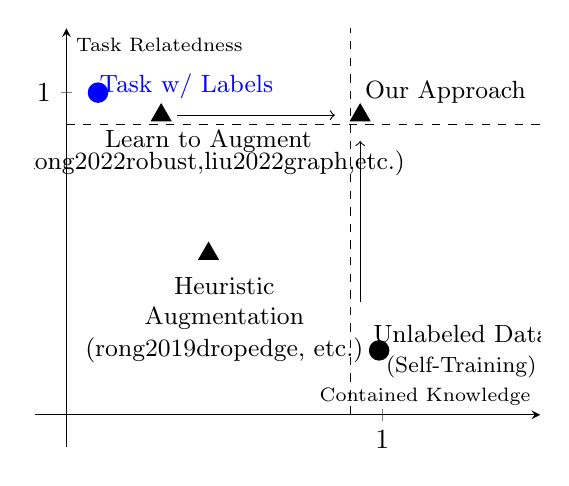
\begin{tikzpicture}
    \begin{axis}
    [
        legend pos= north east,
        axis lines = center,
        domain=-1:2,
        xlabel={\scriptsize Contained Knowledge},
        xmin=-0.1,
        xmax=1.5,
        xtick={0, 1},
        ylabel={\scriptsize Task Relatedness},
        ymin=-0.1,
        ytick={0, 1},
        ymax=1.2,
    ]
    % purple pentagon
    \addplot[only marks, color=black, mark=triangle*, mark size=4pt] coordinates { (0.93,0.93) };
    \node[] at (axis cs: 1.2, 1.0) {\textcolor{black}{\small Our Approach}};

    
    % magenta
    \addplot[only marks, color=black, mark=triangle*,mark size=4pt] coordinates {(0.3,0.93)};
    \node[] at (axis cs: 0.45,0.85) {\textcolor{black}{\small Learn to Augment}};
    \node[] at (axis cs: 0.45,0.78) {\small (\citeauthor{kong2022robust},\citeauthor{liu2022graph},etc.)};
    
    % cyan
    \addplot[only marks, color=black, mark=triangle*,mark size=4pt]
        coordinates {(0.45,0.5) };
    \node[] at (axis cs: 0.5,0.4) {\textcolor{black}{\small Heuristic}};
    \node[] at (axis cs: 0.5,0.3) {\textcolor{black}{\small Augmentation}};
    \node[] at (axis cs: 0.5,0.2) {\textcolor{black}{\small (\citeauthor{rong2019dropedge}, etc.)}};
    
    % red square
    \addplot[only marks, color=blue, mark=*, mark size=3.5pt]
        coordinates {(0.1,1)};
    \node[] at (axis cs: 0.38,1.02) {\textcolor{blue}{\small Task w/ Labels}};

    % color=blue
    \addplot[only marks, color=black, mark=*, mark size=3.5pt]
        coordinates {(0.99,0.2) };
    \node[] at (axis cs: 1.25,0.25) {\textcolor{black}{\small Unlabeled Data}};
    \node[] at (axis cs: 1.25,0.15) {\textcolor{black}{\footnotesize (Self-Training)}};
    
    \draw [dashed] (0.9,0) -- (0.9,1.2);
    \draw [dashed] (0,0.9) -- (1.5,0.9);
    \draw[->](axis cs: 0.35,0.93)--(axis cs: 0.85,0.93);
    \draw[->](axis cs: 0.93,0.35)--(axis cs: 0.93,0.85);
    % \draw[->](unlabeled)--(ours);
    \end{axis}
\end{tikzpicture}}
%     \vspace{-0.2in}
%     \caption{Qualitative relationship of graphs from different data-centric approach on the task closeness and contained knowledge.
%      } 
%     \label{fig: info relationship}
%     \vspace{-0.3in}
% \end{figure}

\section{Additional Related Work on Data-Centric Approach}\label{add:sec:related}
\paragraph{Data Augmentation}
Data augmentation creates new examples with preserved labels but uses no unlabeled data~\citep{shorten2019survey,kashefi2020quantifying,balestriero2022effects}. Examples of heuristic data augmentation techniques include flipping, distorting, and rotating images~\citep{shorten2019survey}, using lexical substitution, inserting words, and shuffling sentences in texts~\citep{kashefi2020quantifying}, and deleting nodes and dropping edges in graphs~\citep{zhao2022graph}. While human knowledge can be used to improve data diversity and reduce over-fitting in heuristic methods, it is difficult to use a single heuristic method to preserve the different labels for different tasks~\citep{balestriero2022effects, cubuk2019autoaugment}. So, automated augmentation~\citep{cubuk2019autoaugment} learned from data to search for the best policy to combine a bunch of predefined heuristic augmentations. Generation models~\citep{antoniou2017data,bowles2018gan,han2022g} create in-class examples. Other learning ideas such as \textsc{FATTEN}~\citep{liu2018feature} and \textsc{GREA}~\citep{liu2022graph} learned to split the latent space for data augmentation. However, learning and augmenting from insufficient labels at the same time may limit the diversity of new examples and cause over-fitting. \method leverages unlabeled data to avoid them.

\paragraph{Relationship between Data-Centric Approaches} 
\begin{wrapfigure}{r}{5.5cm}
\caption{Qualitative relationship of graphs from different data-centric approach on the task relatedness and contained knowledge.}\label{fig: info relationship}
\resizebox{.8\linewidth}{!}{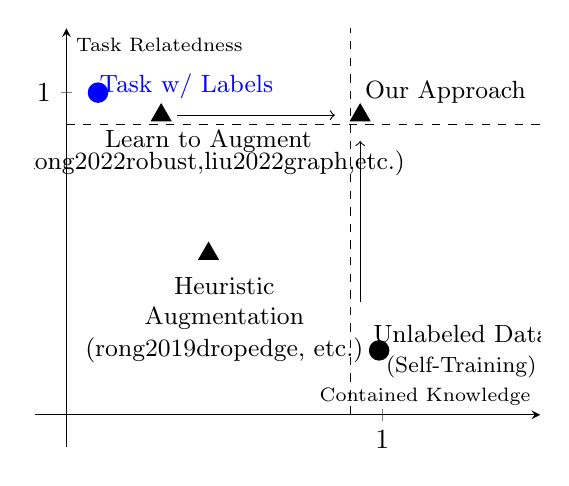
\begin{tikzpicture}
    \begin{axis}
    [
        legend pos= north east,
        axis lines = center,
        domain=-1:2,
        xlabel={\scriptsize Contained Knowledge},
        xmin=-0.1,
        xmax=1.5,
        xtick={0, 1},
        ylabel={\scriptsize Task Relatedness},
        ymin=-0.1,
        ytick={0, 1},
        ymax=1.2,
    ]
    % purple pentagon
    \addplot[only marks, color=black, mark=triangle*, mark size=4pt] coordinates { (0.93,0.93) };
    \node[] at (axis cs: 1.2, 1.0) {\textcolor{black}{\small Our Approach}};

    
    % magenta
    \addplot[only marks, color=black, mark=triangle*,mark size=4pt] coordinates {(0.3,0.93)};
    \node[] at (axis cs: 0.45,0.85) {\textcolor{black}{\small Learn to Augment}};
    \node[] at (axis cs: 0.45,0.78) {\small (\citeauthor{kong2022robust},\citeauthor{liu2022graph},etc.)};
    
    % cyan
    \addplot[only marks, color=black, mark=triangle*,mark size=4pt]
        coordinates {(0.45,0.5) };
    \node[] at (axis cs: 0.5,0.4) {\textcolor{black}{\small Heuristic}};
    \node[] at (axis cs: 0.5,0.3) {\textcolor{black}{\small Augmentation}};
    \node[] at (axis cs: 0.5,0.2) {\textcolor{black}{\small (\citeauthor{rong2019dropedge}, etc.)}};
    
    % red square
    \addplot[only marks, color=blue, mark=*, mark size=3.5pt]
        coordinates {(0.1,1)};
    \node[] at (axis cs: 0.38,1.02) {\textcolor{blue}{\small Task w/ Labels}};

    % color=blue
    \addplot[only marks, color=black, mark=*, mark size=3.5pt]
        coordinates {(0.99,0.2) };
    \node[] at (axis cs: 1.25,0.25) {\textcolor{black}{\small Unlabeled Data}};
    \node[] at (axis cs: 1.25,0.15) {\textcolor{black}{\footnotesize (Self-Training)}};
    
    \draw [dashed] (0.9,0) -- (0.9,1.2);
    \draw [dashed] (0,0.9) -- (1.5,0.9);
    \draw[->](axis cs: 0.35,0.93)--(axis cs: 0.85,0.93);
    \draw[->](axis cs: 0.93,0.35)--(axis cs: 0.93,0.85);
    % \draw[->](unlabeled)--(ours);
    \end{axis}
\end{tikzpicture}}
\end{wrapfigure} 
As presented in~\cref{fig: info relationship}, perturb edges, delete nodes and mask attributes~\citep{rong2019dropedge,trivedianalyzing} for graphs are some heuristic ways for data augmentation. The augmented knowledge from them is mainly controlled by human prior knowledge on the perturbations and it often fails to be close to the task, \ie, random perturbations hardly preserve labels for the augmented graphs. The learning to augment approaches learn from labeled graphs to perturb graph structures~\citep{luo2022automated}, to estimate graphons for different classes~\citep{han2022g}, or to split the latent space for augmentation~\citep{liu2022graph}. Although these approaches could preserve labels for the augmented graphs, they introduce less extra knowledge to improve the model prediction. In summary, graph data augmentation is effective in expanding knowledge for limited labels, but it makes no use of unlabeled graphs. Besides, the diversity and richness of the domain knowledge from augmented graphs are far from that contained in a large number of unlabeled graphs. To learn from unlabeled graphs, data-centric approaches like the self-training is assumed to be useful when the unlabeled and labeled data are from the same source. It is less studied when we have a single unified unlabeled source for different tasks.
% If we assign pseudo-labels for material-related properties to drug-related unlabeled graphs or vice versa, it could negatively impact the model performance. 

\section{Additional Method Details}
\subsection{Upper bounding the mutual information}
In~\cref{eq:upper bound infonce}, we use a leave-one-out variant of InfoNCE ($\I_\text{bound}$) to derive the upper bound of mutual information. We summarize the derivation~\citep{poole2019variational} here.
\begin{equation}\label{eq:add derivation mi upper bound}
    \begin{split}
        \mathcal{I}_1(G^\prime;G) & = \mathbb{E}_{p (G, G^\prime)} \left[ \operatorname{log} \frac{p(G^\prime|G)}{p(G^\prime)} \right] \\
        & = \mathbb{E}_{p (G, G^\prime)} \left[ \operatorname{log} \frac{p(G^\prime|G) q(G^\prime)}{q(G^\prime) p(G^\prime)} \right] \\
        & = \mathbb{E}_{p (G, G^\prime)} \left[ \operatorname{log} \frac{p(G^\prime|G)}{q(G^\prime)} \right] - \operatorname{KL} (p(G^\prime) || q(G^\prime) ) \\
        & \leq \mathbb{E}_{p (G, G^\prime)} \left[ \operatorname{log} \frac{p(G^\prime|G)}{q(G^\prime)} \right]
        % \\ & = \mathbb{E}_{p(G)} \left[\operatorname{KL} (p(G^\prime| G) || q(G^\prime)) \right]
    \end{split}    
\end{equation}
The intractable upper bound is minimized when the variational approximation $q(G^\prime)$ matches the true marginal $p(G^\prime)$~\citep{poole2019variational}. 
% InfoNCE assumes the density ratio is proportional to $\frac{p(G^\prime|G)}{p(G^\prime)}$. 
For each $G_i$, its augmented output $G_i^\prime$, and $M-1$ negative examples with different labels, we could approximate $q(G_i^\prime) = \frac{1}{M-1} \sum_{j \neq i} p(G_i^\prime | G_j)$. So, we have
\begin{equation}
    \begin{split}
        \mathcal{I}_1(G^\prime_i, G_i) 
        & \leq  \operatorname{log} \frac{p(G_i^\prime| G_i)}{\frac{1}{K-1} \sum_{j=1, j\neq i}^M p(G_i^\prime | G_j)}
        \\ & = \operatorname{log} \frac{p(G_i^\prime| G_i)}{\sum_{j=1, j\neq i}^M p(G_i^\prime | G_j)} + \operatorname{log} (M-1)
        % \\ & \leq \operatorname{log} \frac{p(G_i^\prime| G_i)}{\sum_{k=1, k\neq i}^K p(G_i^\prime | G_k)}
        \\ & = \I_\text{bound} (G_i^\prime; G_i) + \text{constant}
    \end{split}
\end{equation}

\subsection{Extraction of Statistical Features on Graphs}\label{add:sec:raw feature}
For each molecule and polymer graph, we concatenate the following vectors or values for statistical feature extraction.
\begin{compactitem}
    \item the sum of the degree in the graph;
    \item the vector indicating the distribution of atom types;
    \item the vector containing the maximum, minimum and mean values of atoms weights in a molecule or polymer;
    \item the vector containing the maximum, minimum, and mean values of bond valence.
\end{compactitem}
For each protein-protein interaction ego-graph in the biology field, we use the sorted vector of node degree distribution in the graph as the statistical features.

\subsection{Technical Details for Graph Data Augmentation with Diffusion Model}\label{add:method:tech}

\paragraph{The Lookup Table from Atom Type to Node Embedding Space}
Given a graph $G$, we assume the node feature matrix on the graph is $\mathbf{X} \in \mathbb{R}^{n \times F_\text{n}}$, where $n$ is the number of nodes. The edge feature matrix is $\mathbf{E} \in \mathbb{R}^{m \times F_\text{e}}$, where $m$ is the number of edges. There are two ways for $G$ to represent the graph structure in practice. We can use either the dense adjacency matrix $\mathbf{A} \in \mathbb{R}^{n \times n}$ or sparse edge index $\mathbf{I}_e \in \mathbb{R}^{2 \times m}$. The diffusion model~\citep{jo2022score} on graphs prefers the former, which is more straightforward for graph generations. The prediction model prefers the latter because of its flexibility, and less computational cost and time. The transformation between two types of graph structure representation takes additional time. Particularly for molecular graphs, the node features used for generation (one-hot encoding of the atom type) and for prediction (see the official package of OGBG~\footnote{\url{https://github.com/snap-stanford/ogb/blob/master/ogb/utils/features.py}} for details) are different, which introduces extra time to process the graph data. For details, we (1) first need to extract discrete node attributes given the atom type and its neighborhoods; (2) we then need to use an embedding table to embed node attributes in a continuous embedding space; (3) the embedding features of nodes with their graph structure are inputted into the graph neural networks to get the latent representation for nodes. The reverse process for data augmentation in \method may need to repeatedly process graph data with steps (1) and (2). It introduces additional time. So, we build up a lookup table to directly map the atom type to the node embedding. To achieve it, we average the node attributes for the same type of node within the batch. We then use the continuous node attributes as weights to average the corresponding node embedding according to the embedding table.

\paragraph{Instantiations of SDE on Graphs} According to~\citet{song2020score}, we use the Variance Exploding (VE) SDE for the diffusion process. Given the minimal noise $\sigma_{\min}$ and the maximal noise $\sigma_{\max}$, the VE SDE is:
\begin{equation}
\mathrm{d} G =\sigma_{\min }\left(\frac{\sigma_{\max }}{\sigma_{\min }}\right)^t \sqrt{2 \log \frac{\sigma_{\max }}{\sigma_{\min }}} \mathrm{d} \mathbf{w}, \quad t \in(0,1]
\end{equation}
% \begin{equation}
% G^{(t)} - G^{(t-1)} = \sqrt{(\sigma^{(t)})^2 - (\sigma^{(t-1)})^2} \cdot \mathbf{z}^{(t-1)}, \quad \quad t=1,\cdots, N_T 
% \end{equation}
% where $\mathbf{z}^{(t)} \sim \mathcal{N} (\mathbf{0}, \mathbf{I})$ 
The perturbation kernel is derived~\citep{song2020score} as:
\begin{equation}
p_{0 t}(G^{(t)} \mid G^{(0)})=\mathcal{N}\left(G^{(t)} ; G^{(0)}, \sigma_{\min }^2\left(\frac{\sigma_{\max }}{\sigma_{\min }}\right)^{2 t} \mathbf{I}\right), \quad t \in(0,1]
\end{equation}

On graphs, we follow~\citet{jo2022score} to separate the perturbation of adjacency matrix and node features:
\begin{equation}
    p_{0 t}(G^{(t)} \mid G^{(0)}) = p_{0 t}(\mathbf{A}^{(t)} \mid \mathbf{A}^{(0)}) p_{0 t}(\mathbf{X}^{(t)} \mid \mathbf{X}^{(0)}).
\end{equation}


\paragraph{The Sampling Algorithm in the Reverse Process for Graph Data Augmentation} We adapt the Predictor-Corrector (PC) samplers for the graph data augmentation in the reverse process. The algorithm is shown in~\cref{alg:diffusion augmentation}.
\begin{algorithm}[H]
   \caption{Diffusion-Based Graph Augmentation with PC Sampling}
   \small
   \label{alg:diffusion augmentation}
   \def\bfX{\mathbf{X}}
   \def\bfz{\mathbf{z}}
   \def\bfI{\mathbf{I}}
   \def\mclN{\mathcal{N}}
\begin{algorithmic}
    % \STATE $\mathbf{z}_0 \sim  \mclN(\mathbf{0}, \bfI)$
    % \STATE $\mathbf{X}^{(D)} \gets \mathbf{X} + \mathbf{z}_0; \quad \mathbf{A}^{(D)} \gets \mathbf{A} + \mathbf{z}_0$
    \STATE {\bfseries Input:} Graph $G$ with node feature $\mathbf{X}$ and adjacency matrix $\mathbf{A}$, the denoising function for node feature $\mathbf{s}_{\mathbf{X}}$ and adjacency matrix $\mathbf{s}_{\mathbf{A}}$, the fine-tune loss $\mathcal{L}_\textbf{aug}$, Lagevin MCMC step size $\beta$,  scaling coefficient $\epsilon_1$
    \STATE $\mathbf{A}^{(D)} \gets \mathbf{A} + \mathbf{z}_A $; \quad $\mathbf{z}_A \sim \mclN(\mathbf{0}, \bfI)$
    \STATE $\mathbf{X}^{(D)} \gets \mathbf{X} + \mathbf{z}_X $; \quad $\mathbf{z}_X \sim \mclN(\mathbf{0}, \bfI)$
    
   \FOR{$t=D-1$ {\bfseries to}  $0$}
    \STATE $\hat{G}_{(t+1)} \sim p_{0 t+1} ( \hat{G}_{(t+1)} |G^{(t+1)}) $ \COMMENT{inner-loop sampling with another PC sampler}
    
    \STATE $ \mathbf{S}_A = \frac{1}{2} \mathbf{s}_{\mathbf{A}}(G^{(t+1)}, t+1) - \frac{1}{2} 
    \alpha \nabla_{\mathbf{A}^{(t)}} \mathcal{L}_\textbf{aug}(\hat{G}_{(t+1)})$
    
    \STATE  $ \mathbf{S}_X = \frac{1}{2} \mathbf{s}_{\mathbf{X}}(G^{(t+1)}, t+1) - \frac{1}{2} 
    \alpha \nabla_{\mathbf{X}^{(t)}} \mathcal{L}_\textbf{aug}(\hat{G}_{(t+1)})$
    
    \STATE $\tilde{\mathbf{A}}^{(t)} \gets \mathbf{A}^{(t+1)} + g(t)^2 \mathbf{S}_A + g(t) \mathbf{z}_A $; \quad $\mathbf{z}_A \sim \mclN(\mathbf{0}, \bfI)$ \COMMENT{Predictor for adjacency matrix}
    \STATE $\tilde{\mathbf{X}}^{(t)} \gets \mathbf{X}^{(t+1)} +  g(t)^2 \mathbf{S}_X  + g(t) \mathbf{z}_X $; \quad $\mathbf{z}_X \sim \mclN(\mathbf{0}, \bfI)$ \COMMENT{Predictor for node features}
    \STATE $\mathbf{A}^{(t)} \gets \tilde{\mathbf{A}}^{(t)} + \frac{\beta}{2} \mathbf{S}_A + \epsilon_1 \sqrt{\beta} \mathbf{z}_A $; \quad $\mathbf{z}_A \sim \mclN(\mathbf{0}, \bfI)$ \COMMENT{Corrector for adjacency matrix}
    \STATE $\mathbf{X}^{(t)} \gets \tilde{\mathbf{X}}^{(t)} + \frac{\beta}{2} \mathbf{S}_X  + \epsilon_1 \sqrt{\beta} \mathbf{z}_X $; \quad $\mathbf{z}_X \sim \mclN(\mathbf{0}, \bfI)$ \COMMENT{Corrector for node features}

     % \FOR{$j=1$ {\bfseries to} $M$}
     %    \STATE $z \sim {N}(0, I)$
     %    \STATE{$G_{i} \gets G_{i} + \epsilon_i S(G_{i}, \sigma_{i}) + \sqrt{2\epsilon_i} z$}
     % \ENDFOR
   \ENDFOR
   \STATE {return} $G^\prime  = ( \mathbf{A}^{(0)}, \mathbf{X}^{(0)})$
\end{algorithmic}
\end{algorithm}




\section{Additional Experiments Set-ups}\label{sec: add exp setups}
We perform experiments on 15 datasets, including eight classification and seven regression tasks from chemistry, material science, and biology. We use Area under the ROC curve (AUC) for classification performance and mean absolute error (MAE) for regression.
\subsection{Molecule Classification and Regression Tasks}
Seven molecule classification and three molecule regression tasks are from open graph benchmark~\citep{hu2020open}. They were originally collected by MoleculeNet~\citep{wu2018moleculenet} and used to predict molecule properties. They include (1) inhibition to HIV virus replication in \hiv, (2) toxicological properties of 617 types in \toxcast, (3) toxicity measurements such as nuclear receptors and stress response in \toxt, (4) blood–brain barrier permeability in \bbbp, (5) inhibition to human $\beta$-secretase 1 in \bace, (6) FDA approval status or failed clinical trial in \clintox, (7) having drug side effects of 27 system organ classes in \sider, (8) predicting the property of lipophilicity in \lipo, (9) predicting the water solubility ($\log$ solubility in mols per litre) from chemical structures in \esol, (10) predicting the hydration free energy of molecules in water in \freesolv.
For all molecule datasets, we use the scaffold splitting procedure as the open graph benchmark adopted \citep{hu2020open}. It attempts to separate structurally different molecules into different subsets, which provides a more realistic estimate of model performance in experiments~\citep{wu2018moleculenet}.

\subsection{Polymer Regression Tasks}
Four polymer regression tasks include \glass, \melting, \thermal, and \oxygen. They are used to predict different polymer properties such as \emph{glass transition temperature} ($^\circ$C), \emph{melting temperature} ($^\circ$C), \emph{thermal conductivity} (W/mK) and \emph{oxygen permeability} (Barrer). \glass and \melting are collected from PolyInfo, which is the largest web-based polymer database \citep{otsuka2011polyinfo}. The \thermal dataset is from molecular dynamics simulation and is an extension from the dataset used in~\citep{ma2022machine}. The \oxygen dataset is created from the Membrane Society of Australasia portal,
consisting of a variety of gas permeability data \citep{thornton2012polymer}. Since a polymer is built from repeated units, researchers often use a single unit graph with polymerization points as polymer graphs to predict properties. Different from molecular graphs, two polymerization points are two special nodes (see ``$*$'' in \cref{fig:implementation}), indicating the polymerization of monomers \citep{cormack2004molecularly}. For all the polymer tasks, we randomly split by 60\%/10\%/30\% for training, validation, and test.

% Particularly, \textbf{tasks used in \cref{fig:compare gnn runs}} are hiv (\hiv), bace (\bace), bbbp (\bbbp), clintox (\clintox), sider (\sider), tox21 (\toxt), toxcast (\toxcast), oxygen (\oxygen), melting (\melting), and glass (\glass).

\subsection{Protein Classification Task}
An additional task is protein function prediction using protein-protein interaction graphs~\citep{hu2019strategies}. A node is a protein without attributes, an edge is a relation type between two proteins such as co-expression and co-occurrence. In our \method, we treat all the relations as the undirected edge without attributes.


\subsection{Baselines and Implementation}
When implementing \gin~\citep{xu2018powerful}, we tune its hyper-parameters for different tasks with an early stop on the validation set. We generally implement pre-training baselines following their own setting. For molecule and polymer property prediction and protein function prediction, the pre-trained \gin models with self-supervised tasks such as \edgepred, \attrmask, \contextpred in~\citep{hu2019strategies}, \infomax~\citep{velickovic2019deep} are available. So we directly use them. For other self-supervised methods, we implement their codes with default hyper-parameters. Following their settings, we use 2M ZINC15~\citep{sterling2015zinc} to pre-train \gin models for molecule and polymer property prediction. We use 306K unlabeled protein-protein interaction ego-networks~\citep{hu2019strategies} to pre-train the \gin for the downstream protein function property prediction. For self-training with real unlabeled graphs and \infograph~\citep{sun2019infograph}, we use 113K QM9~\citep{ramakrishnan2014quantum}. For self-training with generated unlabeled graphs, we train the diffusion model~\citep{jo2022score} on the real QM9 dataset and then produce the same number of generated unlabeled graphs. To train the diffusion model in our \method, we also use QM9~\citep{ramakrishnan2014quantum}.

% \begin{table}[t]
\centering
\footnotesize
\setlength{\tabcolsep}{4pt} 
\begin{tabular}{lccccc}
\toprule
 & \makecell{Visual\\Context} & \makecell{\#Dialog} & \makecell{Avg. \\\#Turn} & \makecell{Avg. Utt. \\Length} & \makecell{\#Tokens}\\
\midrule 
BST~\citep{smith2020can} & \xmark & 7K & 11.2 & 13.6 & 1M\\
ConvAI2~\citep{dinan2020second} & \xmark & 20K & 13.9 & 9.9 & 2.7M \\
ED~\citep{rashkin2018towards} & \xmark & 25K & 4.3 & 13.7 & 1.5M \\
WOW~\citep{dinan2018wizard} & \xmark & 22K & 9.1 & 16.4 & 3.3M\\
WOI~\citep{komeili2021internet} & \xmark & 9.5K & 10.9 & 13.9 & 1.4M\\
SODA~\citep{kim2022soda} & \xmark & 1.5M & 7.6 & 16.1 & 183M\\
ImageChat~\citep{shuster2018image} & \cmark & 100K & 3.0 & 9.7 & 2.9M \\
OVD2.0~\citep{wang2021openvidial} & \cmark & 116K & \textbf{48.7} & 6.3  & 35.6M\\
MMD~\citep{feng2022mmdialog} & \cmark & 1M & 4.5 & 15.9 & 71.5M \\
\midrule
\datasetName & \cmark & \textbf{18M} & 3.0 & \textbf{19.7} & \textbf{1.06B}\\
\bottomrule
\end{tabular}
\caption {
Statistics of \datasetNameNoEmoji compared to other open-domain dialogue and visually grounded dialogue dataset. \textit{Utt.} stands for utterance.
}
\label{tab:dataset_statistics}
\end{table}


\section{Additional Experiment Analysis}
% \section{Additional Experiments Results and Analysis}


% \definecolor{LightCyan}{rgb}{0.88,1,1}
% \definecolor{negative}{gray}{0.92}
% \begin{table*}[ht!]
%     \renewcommand{\arraystretch}{1.1}
%     \renewcommand{\tabcolsep}{1.5mm}
%     \caption{\small More results {Mean\scriptsize(Std)} on regression tasks. The best mean is \textbf{bonded}. The best baseline is \underline{underlined}. Results are \colorbox{negative}{highlighted} if unlabeled graphs bring significant negative impacts compared to \gin. The MAE for \thermal is scaled $\times$ 100. }
%     \centering
%     \begin{adjustbox}{width=0.98\textwidth}
%     \begin{tabular}{llccccccc}
%     %%%%%%%%%%%%%%%%% regression results
%     \toprule
%     \multicolumn{2}{c}{} & \multicolumn{3}{c}{{Molecule Regression: RMSE $\downarrow$}} & \multicolumn{4}{c}{{Polymer Regression: RMSE $\downarrow$}} \\
%     \cmidrule[0.4pt](lr){3-5} \cmidrule[0.4pt](lr){6-9}
%     & & \lipo & \esol & \freesolv & \glass & \melting & \thermal & \oxygen\\
%     \multicolumn{2}{c}{\# Training Graphs} & 3,360 & 902 & 513 & 4,303 & 2,189 & 455 & 356 \\
%     \midrule
    
%     & \gin & 0.707{\scriptsize (0.022)} & 1.002{\scriptsize (0.032)} & {\scriptsize (X)} 
%     & X {\scriptsize (XX )} & XX {\scriptsize (XX)} & XX {\scriptsize (XXX)} & XXX{\scriptsize (XXX)}
%     \\

%     \midrule
%     \multirow{7}{*}{\rotatebox{90}{\textit{\fontsize{8pt}{8pt} Self-Supervised}}}
    
%     & \edgepred 
%     & 0.773{\scriptsize (0.012)} & X{\scriptsize (XX )} & {\scriptsize (X)} 
%     & X {\scriptsize (XX )} & XX {\scriptsize (XX)} & XX {\scriptsize (XXX)} & XXX{\scriptsize (XXX)} \\
%     & \attrmask 
%     &  0.757{\scriptsize (0.011)} & X{\scriptsize (XX )} & {\scriptsize (X)} 
%     & X {\scriptsize (XX )} & XX {\scriptsize (XX)} & XX {\scriptsize (XXX)} & XXX{\scriptsize (XXX)} \\
%     & \contextpred 
%     & 0.783{\scriptsize (0.013)} & X{\scriptsize (XX )} & {\scriptsize (X)} 
%     & X {\scriptsize (XX )} & XX {\scriptsize (XX)} & XX {\scriptsize (XXX)} & XXX{\scriptsize (XXX)}\\
%     & \infomax 
%     &  0.752{\scriptsize (0.013)} & X{\scriptsize (XX )} & {\scriptsize (X)} 
%     & X {\scriptsize (XX )} & XX {\scriptsize (XX)} & XX {\scriptsize (XXX)} & XXX{\scriptsize (XXX)} \\
%     & \joao 
%     & 0.770 {\scriptsize (0.010)} & X{\scriptsize (XX )} & {\scriptsize (X)} 
%     & X {\scriptsize (XX )} & XX {\scriptsize (XX)} & XX {\scriptsize (XXX)} & XXX{\scriptsize (XXX)}\\
%     & \graphlog 
%     &  0.759{\scriptsize (0.012)} & X{\scriptsize (XX )} & {\scriptsize (X)} 
%     & X {\scriptsize (XX )} & XX {\scriptsize (XX)} & XX {\scriptsize (XXX)} & XXX{\scriptsize (XXX)} \\
%     & \dsla 
%     &  0.731 {\scriptsize (0.006)} & X{\scriptsize (XX )} & {\scriptsize (X)} 
%     & X {\scriptsize (XX )} & XX {\scriptsize (XX)} & XX {\scriptsize (XXX)} & XXX{\scriptsize (XXX)} \\

%     \midrule
%     \multirow{3}{*}{\rotatebox{90}{\textit{\fontsize{8pt}{8pt} Semi-SL}}}
%     & \infograph 
%     &  0.969{\scriptsize (0.107)} & X{\scriptsize (XX )} & {\scriptsize (X)} 
%     & X {\scriptsize (XX )} & XX {\scriptsize (XX)} & XX {\scriptsize (XXX)} & XXX{\scriptsize (XXX)}  \\
    
%     & \streal 
%     &  0.696{\scriptsize (0.008)} & 1.021{\scriptsize (0.106)} & {\scriptsize (X)} 
%     & X {\scriptsize (XX )} & XX {\scriptsize (XX)} & XX {\scriptsize (XXX)} & XXX{\scriptsize (XXX)} \\
%     & \stgen &
%      0.698{\scriptsize (0.029)} & 0.928{\scriptsize (0.116)} & {\scriptsize (X)} & X {\scriptsize (XX )} & XX {\scriptsize (XX)} & XX {\scriptsize (XXX)} & XXX{\scriptsize (XXX)}\\
%     \midrule
%     \multirow{2}{*}{\rotatebox{90}{\textit{\fontsize{8pt}{8pt} GDA}}} 
    
%     & \flag & 0.693{\scriptsize (0.006)} & X{\scriptsize (XX )} & {\scriptsize (X)} & X {\scriptsize (XX )} & XX {\scriptsize (XX)} & XX {\scriptsize (XXX)} & XXX{\scriptsize (XXX)} \\
%     & \grea & 0.753{\scriptsize (0.038)} & X{\scriptsize (XX )} & {\scriptsize (X)} & X {\scriptsize (XX )} & XX {\scriptsize (XX)} & XX {\scriptsize (XXX)} & XXX{\scriptsize (XXX)}\\

%     \midrule
%     & \method~(Ours)  0.683{\scriptsize (0.014)} & X{\scriptsize (XX )} & {\scriptsize (X)} 
%     & X {\scriptsize (XX )} & XX {\scriptsize (XX)} & XX {\scriptsize (XXX)} & XXX{\scriptsize (XXX)} \\
%     \bottomrule
%     \end{tabular}
%     \end{adjustbox}
%     \vspace{-0.1in}
%     \label{add:tab:more reg results}
% \end{table*}

\subsection{The Power of Diffusion Model to Learn from Unlabeled Graphs}
In~\cref{tab:ablation finetune}, when we replace the 133K QM9 with the 249K ZINC~\citep{jo2022score} to train the diffusion model, which nearly doubles the size of the unlabeled graphs and includes more atom types, we do not observe any additional improvement, and in some cases, even worse performance. It is possible because of the constraint of the current diffusion model's capacity to model the data distribution for a much larger number of more complex graphs. It encourages powerful generative models in the future, which could be directly used to benefit predictive models under the proposed framework.

% Appendix here

% \input{figures/math_fig.tex}
% \section{You \emph{can} have an appendix here.}

% You can have as much text here as you want. The main body must be at most $8$ pages long.
% For the final version, one more page can be added.
% If you want, you can use an appendix like this one, even using the one-column format.
%%%%%%%%%%%%%%%%%%%%%%%%%%%%%%%%%%%%%%%%%%%%%%%%%%%%%%%%%%%%%%%%%%%%%%%%%%%%%%%
%%%%%%%%%%%%%%%%%%%%%%%%%%%%%%%%%%%%%%%%%%%%%%%%%%%%%%%%%%%%%%%%%%%%%%%%%%%%%%%


\end{document}


% This document was modified from the file originally made available by
% Pat Langley and Andrea Danyluk for ICML-2K. This version was created
% by Iain Murray in 2018, and modified by Alexandre Bouchard in
% 2019 and 2021 and by Csaba Szepesvari, Gang Niu and Sivan Sabato in 2022. 
% Previous contributors include Dan Roy, Lise Getoor and Tobias
% Scheffer, which was slightly modified from the 2010 version by
% Thorsten Joachims & Johannes Fuernkranz, slightly modified from the
% 2009 version by Kiri Wagstaff and Sam Roweis's 2008 version, which is
% slightly modified from Prasad Tadepalli's 2007 version which is a
% lightly changed version of the previous year's version by Andrew
% Moore, which was in turn edited from those of Kristian Kersting and
% Codrina Lauth. Alex Smola contributed to the algorithmic style files.
